\documentclass[
10pt, % The default document font size, options: 10pt, 11pt, 12pt
%oneside, % Two side (alternating margins) for binding by default, uncomment to switch to one side
english, % ngerman for German
singlespacing, % Single line spacing, alternatives: onehalfspacing or doublespacing
%draft, % Uncomment to enable draft mode (no pictures, no links, overfull hboxes indicated)
%nolistspacing, % If the document is onehalfspacing or doublespacing, uncomment this to set spacing in lists to single
%liststotoc, % Uncomment to add the list of figures/tables/etc to the table of contents
%toctotoc, % Uncomment to add the main table of contents to the table of contents
%parskip, % Uncomment to add space between paragraphs
%nohyperref, % Uncomment to not load the hyperref package
headsepline, % Uncomment to get a line under the header
%chapterinoneline, % Uncomment to place the chapter title next to the number on one line
%consistentlayout, % Uncomment to change the layout of the declaration, abstract and acknowledgements pages to match the default layout
]{report}
% \setlength{\parskip}{\baselineskip}%
\setlength{\parskip}{5pt}
\setlength{\parindent}{0pt}

%Goldsmiths packages
\usepackage[utf8]{inputenc} 
\usepackage[T1]{fontenc} 
\usepackage{mathpazo}
\usepackage[autostyle=true]{csquotes} 
\usepackage{tabulary}

\usepackage{caption}
\usepackage{subcaption}

\usepackage[utf8]{inputenc}
\usepackage[margin=1.26in]{geometry}
\usepackage{lipsum}
\usepackage{graphicx}
\usepackage{adjustbox}
\usepackage{natbib}
\usepackage{amsmath}

\setcounter{tocdepth}{4}
\setcounter{secnumdepth}{4}

\usepackage{float}
% %Imports needed for displaying code
% \usepackage{listings}
% \usepackage{color}
% \definecolor{dkgreen}{rgb}{0,0.6,0}
% \definecolor{gray}{rgb}{0.5,0.5,0.5}
% \definecolor{mauve}{rgb}{0.58,0,0.82}


% %Stuff for the timeline
% \usepackage[utf8]{inputenc}
% \usepackage[TS1,T1]{fontenc}
% \usepackage{fourier, heuristica}
% \usepackage{array, booktabs}
% \usepackage{graphicx}
% \usepackage[x11names,table]{xcolor}
% \usepackage{caption}
% \DeclareCaptionFont{blue}{\color{LightSteelBlue3}}

% \lstset{frame=tb,
%   language=Java,
%   aboveskip=3mm,
%   belowskip=3mm,
%   showstringspaces=false,
%   columns=flexible,
%   basicstyle={\small\ttfamily},
%   numbers=none,
%   numberstyle=\tiny\color{gray},
%   keywordstyle=\color{blue},
%   commentstyle=\color{dkgreen},
%   stringstyle=\color{mauve},
%   breaklines=true,
%   breakatwhitespace=true,
%   tabsize=3
% }
% \input{formatPackage}
\graphicspath{ {./figures/} }


%----------------------------------------------------------------------------------------
%	THESIS INFORMATION
%----------------------------------------------------------------------------------------
% \usepackage[Bjornstrup]{fncychap}





\begin{document}
    
    
    \thesistitle{Deep Image Colourisation:  comparing AutoEncoders and Conditional Adversarial Networks}
    \degree{BSc Computer Science Degree} % Your degree name, this is used in the title page and abstract, print it elsewhere with \degreename
    \author{Muneeb \textsc{Rehman}} % Your name, this is used in the title page and abstract, print it elsewhere with \authorname
    \addresses{} % Your address, this is not currently used anywhere in the template, print it elsewhere with \addressname
    
    \subject{Computer Science} % Your subject area, this is not currently used anywhere in the template, print it elsewhere with \subjectname
    \keywords{Image Colourisation, Convolutional Neural networks, AutoEncoders, cGAN, evaluation} % Keywords for your thesis, this is not currently used anywhere in the template, print it elsewhere with \keywordnames
    \college{Goldsmiths College }
    %\college{\href{http://www.goldsmiths.com}{Goldsmiths College}} % Your college's name and URL, this is used in the title page and abstract, print it elsewhere with \collegename
    \university{University of London}
    %\university{\href{http://www.university.com}{University Name}} % Your university's name and URL, this is used in the title page and abstract, print it elsewhere with \univname
    \department{Computing Department}
    %\department{\href{http://doc.gold.ac.uk}{Computing Department}} % Your department's name and URL, this is used in the title page and abstract, print it elsewhere with \deptname
    %\group{\href{http://researchgroup.university.com}{Research Group Name}} % Your research group's name and URL, this is used in the title page, print it elsewhere with \groupname


    \rmfamily
    \pagenumbering{roman}
    %TC:ignore 
    
    \begin{titlepage}

\newcommand{\HRule}{\rule{\linewidth}{0.5mm}} % Defines a new command for the horizontal lines, change thickness here

%----------------------------------------------------------------------------------------
%	LOGO SECTION
%----------------------------------------------------------------------------------------
\centering

\includegraphics[width=4cm]{sections/figures/goldsmiths_logo.png}\\[1cm] % Include a department/university logo - this will require the graphicx package
\textsc{\LARGE Goldsmiths, University Of London}\\[1.5cm] % Main heading 
%----------------------------------------------------------------------------------------

\center % Center everything on the page

%----------------------------------------------------------------------------------------
%	HEADING SECTIONS
%----------------------------------------------------------------------------------------

\textsc{\LARGE Final Year Project}\\[1.5cm] 


%----------------------------------------------------------------------------------------
%	TITLE SECTION
%----------------------------------------------------------------------------------------
\makeatletter
\HRule \\[0.4cm]
{ \huge \bfseries Deep Image Colourisation:  comparing AutoEncoders and Conditional Adversarial Networks}\\[0.4cm]% Title of your document
\HRule \\[1.5cm]
 
%----------------------------------------------------------------------------------------
%	AUTHOR SECTION
%----------------------------------------------------------------------------------------

\begin{minipage}{0.4\textwidth}
\begin{flushleft} \large
\emph{Author:}\\
Muneeb Rehman 



\end{flushleft}
\end{minipage}
~
\begin{minipage}{0.4\textwidth}
\begin{flushright} \large
\emph{Supervisor:} \\
Dr. Tim Blackwell
\end{flushright}
\end{minipage}\\[2cm]
\makeatother



% \vspace{1.0in}

\vfill

\large \textit{A thesis submitted in fulfillment of the requirements\\ for \degreename}\\[0.3cm] % University requirement text

%----------------------------------------------------------------------------------------
%	DATE SECTION
%----------------------------------------------------------------------------------------
\vfill
{\large \today}\\[2cm] % Date, change the \today to a set date if you want to be precise



\end{titlepage}
\cleardoublepage
    % \chapter*{Declaration of Authorship}
% I, Muneeb Rehman, declare that except where specific reference is made to the work of others, the contents of this dissertation are original and have not been submitted in whole or in part for consideration for any other degree or 
% qualification in this, or any other university. This dissertation is my own 
% work and contains nothing which is the outcome of work done in collaboration 
% with others, except as specified in the text and Acknowledgements.

\begin{declaration}
\addchaptertocentry{\authorshipname} % Add the declaration to the table of contents
\noindent I, \authorname, declare that this thesis titled, \enquote{\ttitle} and the work presented in it are my own. I confirm that:

\begin{itemize} 
\item Where I have consulted the published work of others, this is always clearly attributed.
\item Where I have quoted from the work of others, the source is always given. With the exception of such quotations, this thesis is entirely my own work.
\item I have acknowledged all main sources of help.
\end{itemize}
 
\noindent Signed: Muneeb Rehman\\
\rule[0.5em]{25em}{0.5pt} % This prints a line for the signature
 
\noindent Date: 05/05/2022\\
\rule[0.5em]{25em}{0.5pt} % This prints a line to write the date
\end{declaration}

\cleardoublepage

    \begin{abstract}
\addchaptertocentry{\abstractname} % Add the abstract to the table of contents

Image colorization is the process of taking a grayscale image and adding color information to it in a way that looks realistic. Early methods for colorization relied on user-guided techniques, such as scribbling and using reference images. However, nowadays deep learning techniques for image colorization have been introduced, which eradicates the need for user guidance. There are several types of deep learning architectures that can achieve image colorization, such as AutoEncoders and conditional adversarial networks. This investigation only focuses on deep learning techniques for image colorization, specifically AutoEncoders and cGANs. The investigation aims to compare the performance between AutoEncoders and cGANs using quantitative metrics. In addition to this, the investigation also looks into whether objective metrics, such as PSNR and SSIM, correlate with human opinion in regard to image colorization and determines which method of evaluation is best suited when analyzing image colorization methods. The limitations suffered from each method and possible future research are also mentioned. The investigation concludes that using objective metrics for evaluation is unreliable for measuring colors from the image and using user studies is the optimal solution. The cGAN models performed overall the best, by producing more realistic colorization and adding a higher variety of colors.

\textbf{Keywords - \keywordnames}
\end{abstract}


    \begin{acknowledgements}
\addchaptertocentry{\acknowledgementname} % Add the acknowledgements to the table of contents
Firstly, I would like to thank my supervisor, Tim Blackwell, for providing me with support and guidance along the way. I would also like to thank my parents for their support throughout my studies.
\end{acknowledgements}

% \chapter*{Acknowledgments}
    \tableofcontents % Prints the main table of contents
    \listoffigures % Prints the list of figures
    \begin{abbreviations}{ll} % Include a list of abbreviations (a table of two columns)

\textbf{ANN} & \textbf{A}rtificial  \textbf{N}eural \textbf{N}etwork\\
\textbf{CNN} & \textbf{C}onvolutional  \textbf{N}eural \textbf{N}etwork\\
\textbf{GAN} & \textbf{G}enerative  \textbf{A}dversarial \textbf{N}etwork\\
\textbf{cGAN} & \textbf{C}onditional  \textbf{G}enerative  \textbf{A}dversarial \textbf{N}etwork\\
\textbf{GFE} & \textbf{G}lobal  \textbf{F}eature \textbf{E}xtractor\\
\textbf{PSNR} & \textbf{P}eak  \textbf{S}ignal to \textbf{N}oise \textbf{R}ationetwork\\
\textbf{SSIM} & \textbf{S}tructural  \textbf{S}imilarity \textbf{I}ndex \textbf{M}easure\\
\end{abbreviations}





% \makeglossaries


% \makeglossaries


% \newacronym{ANN}{ANN}{Artificial Neural Network}
% \newacronym{CNN}{CNN}{Convolutional Neural Network}
% \newacronym{GAN}{GAN}{Generative Adversarial Network}
% \newacronym{cGAN}{cGAN}{Conditional Generative Adversarial Network}
% \newacronym{GFE}{GFE}{Global Feature Extractor}
% \newacronym{PSNR}{PSNR}{Peak Signal-to-noise ratio}




% \begin{center}
% \begin{tabular}{ |c|c| } 
% \hline
% col1 & col2 & col3 \\
% \hline
% \multirow{3}{4em}{Multiple row} & cell2 & cell3 \\ 
% & cell5 & cell6 \\ 
% & cell8 & cell9 \\ 
% \hline
% \end{tabular}
% \end{center}
    %TC:endignore
    

    %Sections

    
\chapter{Introduction}
\pagenumbering{arabic}
\section{Purpose and Motivation}
The main \textbf{purpose} of this report is to investigate various techniques used for the application of image colourisation and restoration purposes using deep learning tactics such as AutoEncoders and Conditional Generative Adversarial Network (cGAN). These purposes may include applying colour to an old black and white image or restoring an old coloured image to its original form as accurately as possible.  

The \textbf{motivation} for my project came from watching historical documentaries that were recently colourised using artificial intelligence. The colourisation added a lot more sense of immersion; it made every human being, every car, every horse, and everything look more real and alive. What was more impressive was that it was all done by AI. This fascinates me because, for the human mind, the idea of image colourisation is a simple task. We learn this from a very early age—to fill in the missing colours from a colouring book, by knowing the fact that the sky is blue, the grass is green, clouds are white, apples are red or green. Using deep learning, we can replicate that mindset for a machine to automate the process of colourising photos for us.

On top of that, I also thought that having such a model would allow it to be a useful tool for users to apply colours to old black and white image artefacts or restore videos and images that have suffered deterioration in quality over time. 

Moreover, AI image colourisation can be used to reveal semantic meaning or details that may have otherwise been left out or lost from the image. Besides that, having an automated colourisation process can eliminate the need to hire an artist (or can be used to assist them) to colourise or restore your photos, as such a model will be able to do what an image restoration artist can, for free and fast.

\section{Aims}
The \textbf{aim} of this project is to determine the best image colourisation method by \textbf{carrying out analysis} of \textbf{deep learning architectures such as AutoEncoders and Conditional Adversarial Networks} using \textbf{quantitative measures such as human assessment and objective metrics}.

In addition to this aim, the project will investigate whether the \textbf{objective measures correlates with human assessment} results and \textbf{determine which measure matters more for the purpose of image colourisation}.

\section{Scope}
The \textbf{scope} of this research project is to conduct an analysis and evaluation of architectures such as AutoEncoders and cGAN for the task of image colourisation, and determine which method is best suited for this task. A total of four existing method architectures will be used for this study. The first two methods are AutoEncoders whereas the second two are cGANs. All methods will be trained using a dataset, Places365 which is split into 60:20:20 for training, testing and validation respectively. PSNR and Naturalness perception study will be the metrics used to evaluate each method's performance in the test set. Visualisations will also be used to showcase the colourisation ability.  


\section{Section Overview}
\textbf{Chapter 2: Background Research}: This chapter goes over the intuition about the history and process of image colourisation, as well as the area of research within deep learning and similar projects.

\textbf{Chapter 3: Methodology} This section of the report will go over the step by step methodology used to conduct my research, including the data preprocessing. Here, I will be describing the methods I have used to experiment with image colourisation.

\textbf{Chapter 3 Research results:} In this chapter, I will be going through the results gathered from the implementation and training. Each method will be tested against unseen test data. Their results will be in the form of visualisations and quantitative metrics used to evaluate each method's performance and determine which class method is best suited for the purpose of image colourisation. In addition to that, I will discuss the results along the way and go over any existing limitations suffered from each method.

\textbf{Chapter 4 Conclusion & future work:} The final chapter of the report will conclude the investigation by going over what has been accomplished along the way but also possible improvements which may yield better results for this investigation as future work.




% \section{Objectives}
% In order to achieve my aims, I will be following a thorough deep learning workflow methodology, where I will iteratively develop and tune and test models until I derive an optimal model. Python will be used to develop the model using the TensorFlow deep learning framework.

    \chapter{Background research}

\section{AI image colourisation}

The problem of automated image colourisation from the previous century did not receive much attention. The process was carried out manually, mostly by artists. Back then, early photography lacked the developing agent which as a consequence made it more prone to quality deterioration due to the conditions of the environment. These environmental factors can be the humidity from the air, dust particles, temperature and mould. Other factors can be due to inappropriate storage, mishandling of images or improper image restoration process \cite{ware1994mechanism}. Additionally, early photography was in black and white, and the need for colourising them was in demand. Image restoration artists were often required to maintain these images and also enhance them (e.g add colourisation). 

It wasn't until this century when in 2004 when Anat Levin and Dani Lischinski proposed an automated solution \cite{Levin2004} that required users to scribble colours on a grayscale image, and then the process will apply the colour to regions across the image. 

\begin{figure}[H]
    \centering
    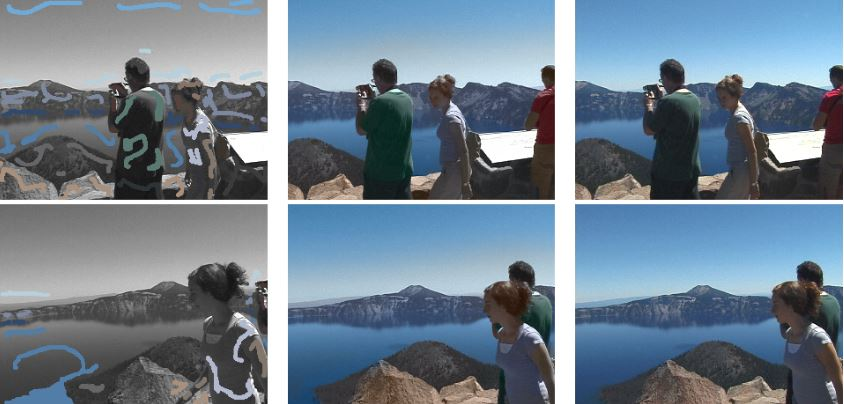
\includegraphics[width=0.6\columnwidth]{sections/figures/scribble_technique_colourisation.JPG}
    \caption{Anat Levin and Dani Lischinski's image colourisation method}
    \label{fig:my_label}
\end{figure}

This in turn significantly reduces the need for human intervention in the process of image colourisation. However, the limitation of Anat Levin and Dani Lischinski's method was that it was considered slow in producing the results. Over time, later research provided more automated methods for image colourisation. Whilst the methods provided by Anat Levin and Dani Lischinksi required one or several referenced images (provided by users or received automatically) as source data. The model learns to transfer colour across regions as shown in figure 2.1. 

On the other hand, newer methods involve a function that learns predictions from colour images from an extensive dataset during training, and the colourisation problem will either be a regression within the continuous colour space or a classification of colours with associated objects in the image. 




\subsection{Image colourisation projects}
This section goes over several existing projects relating to image colourisation.
\subsubsection*{Deoldify}
\addcontentsline{toc}{subsubsection}{Deoldify}
\textbf{Deoldify} is a well known black and white image colourisation library developed by Jason Antic\cite{jantic}. This project uses state of the art techniques such as GANS and has impressive colourisation results. Recently, Deoldify has developed a new type of GAN training method called No-GAN which is a model that addresses the many issues faced by his previous GAN model. A few of these issues are disruptive visual artefacts, bugs and inaccurate colouring. According to Jason Antic, the use of No-Gan has reportedly shown impressive results and achieves realistic colourisation.
\begin{figure}[H]
    \centering
    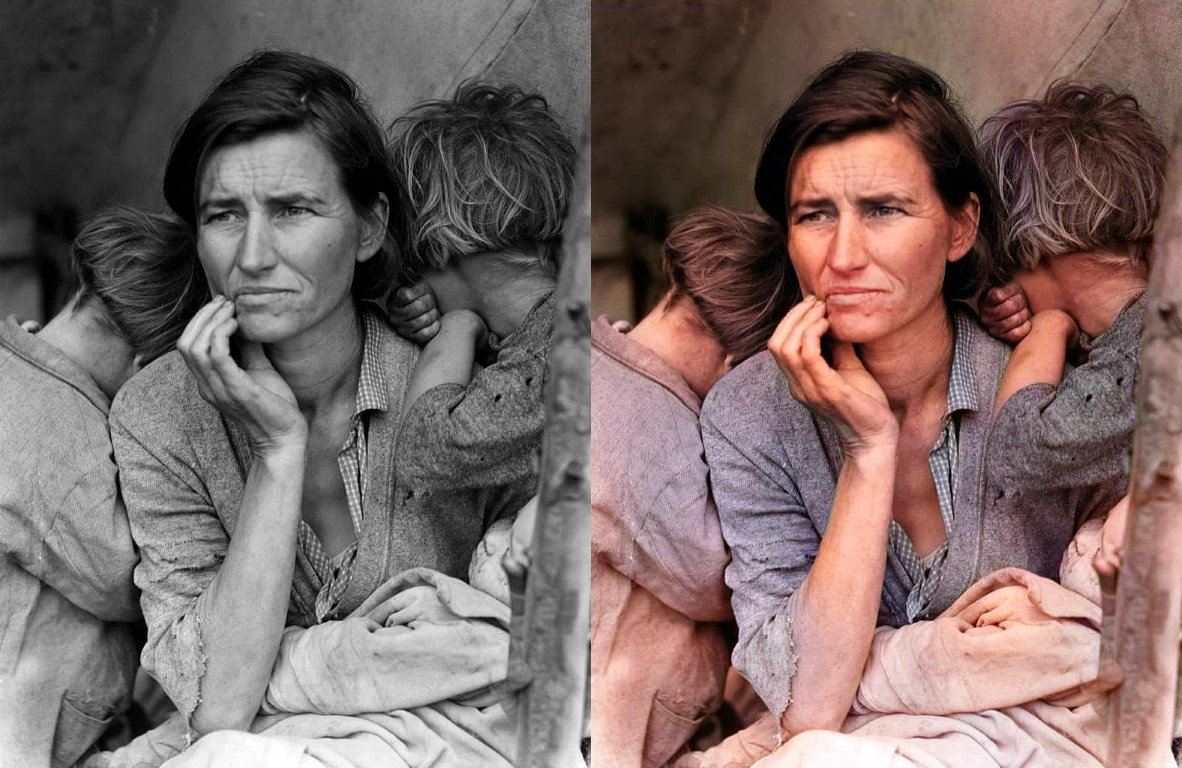
\includegraphics[width=0.7\columnwidth]{sections/figures/deoldify.jpg}
    \caption{Image colourised using Deoldify}
    \label{fig:my_label}
\end{figure}


\subsubsection*{Scribbler}
\addcontentsline{toc}{subsubsection}{Scribbler}
Scribbler (not to be confused with  Anat \& Dani's scribble method) is an interesting technique that involves turning pictures of sketches into realistic images using generative techniques\cite{sangkloy2016scribbler}. Even though their aim doesn't directly align with mine (image colourisation), their model can still generate realistic images with colours. They used a technique similar to \cite{Levin2004}, which involves user guidance by scribbling colours onto a sketch and will systematically apply those colours, whilst at the same time transforming the sketch into a realistic image. Their method is trained using in a GAN manner.
\begin{figure}[H]
    \centering
    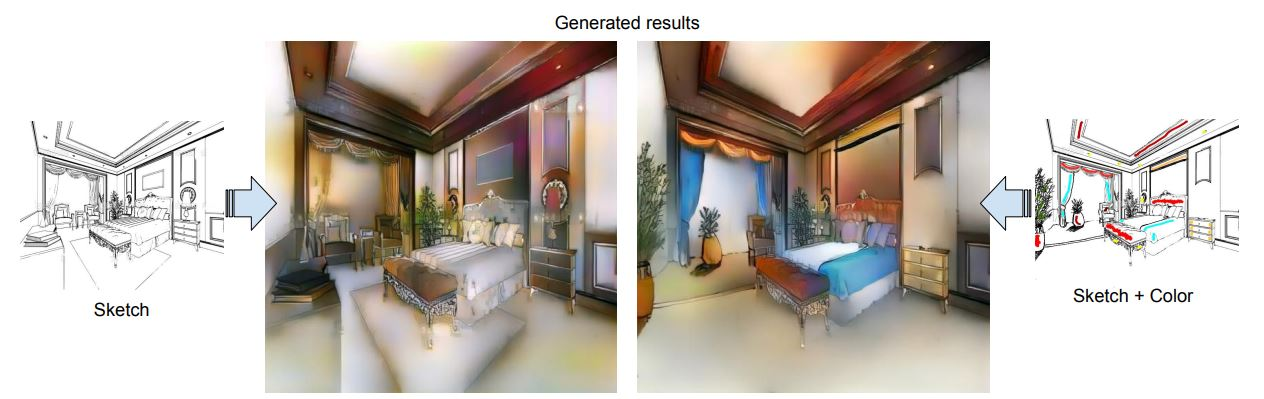
\includegraphics[width=0.7\columnwidth]{sections/figures/scribbler.JPG}
    \caption{Turning sketches into realistic images using Scribbler}
    \label{fig:my_label}
\end{figure}


\subsubsection*{Let there be Color!}
\addcontentsline{toc}{subsubsection}{Let there be Color!}
Similarly, "Let there be Color!" is another project that uses deep learning techniques to colourise black and white images, and is developed by \cite{IizukaSIGGRAPH2016}. They use an AutoEncoder which has been slightly modified to include a global feature extractor model. The addition of this modification meant the colourisation could be more accurate by applying relevant colours of the predicted class of the image. Their model has shown impressive colourisation results, as seen below in figure 2.3:
\begin{figure}[H]
    \centering
    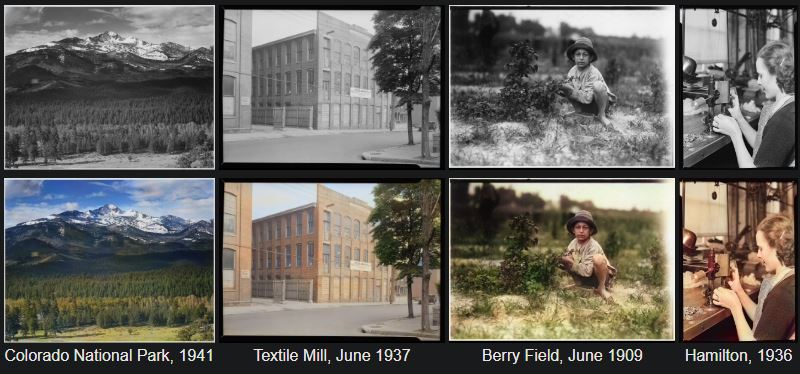
\includegraphics[width=0.7\columnwidth]{sections/figures/LTBC.JPG}
    \caption{Image colourisation results}
    \label{fig:my_label}
\end{figure}

\subsubsection*{End-to-End Image Colourisation}
\addcontentsline{toc}{subsubsection}{Pix2Pix}

The End-to-End conditional GAN-based image colourisation paper by \cite{inproceedings}. They use a conditional GAN architecture which is based on a well known cGAN architecture "Pix2Pix".

\begin{figure}[H]
    \centering
    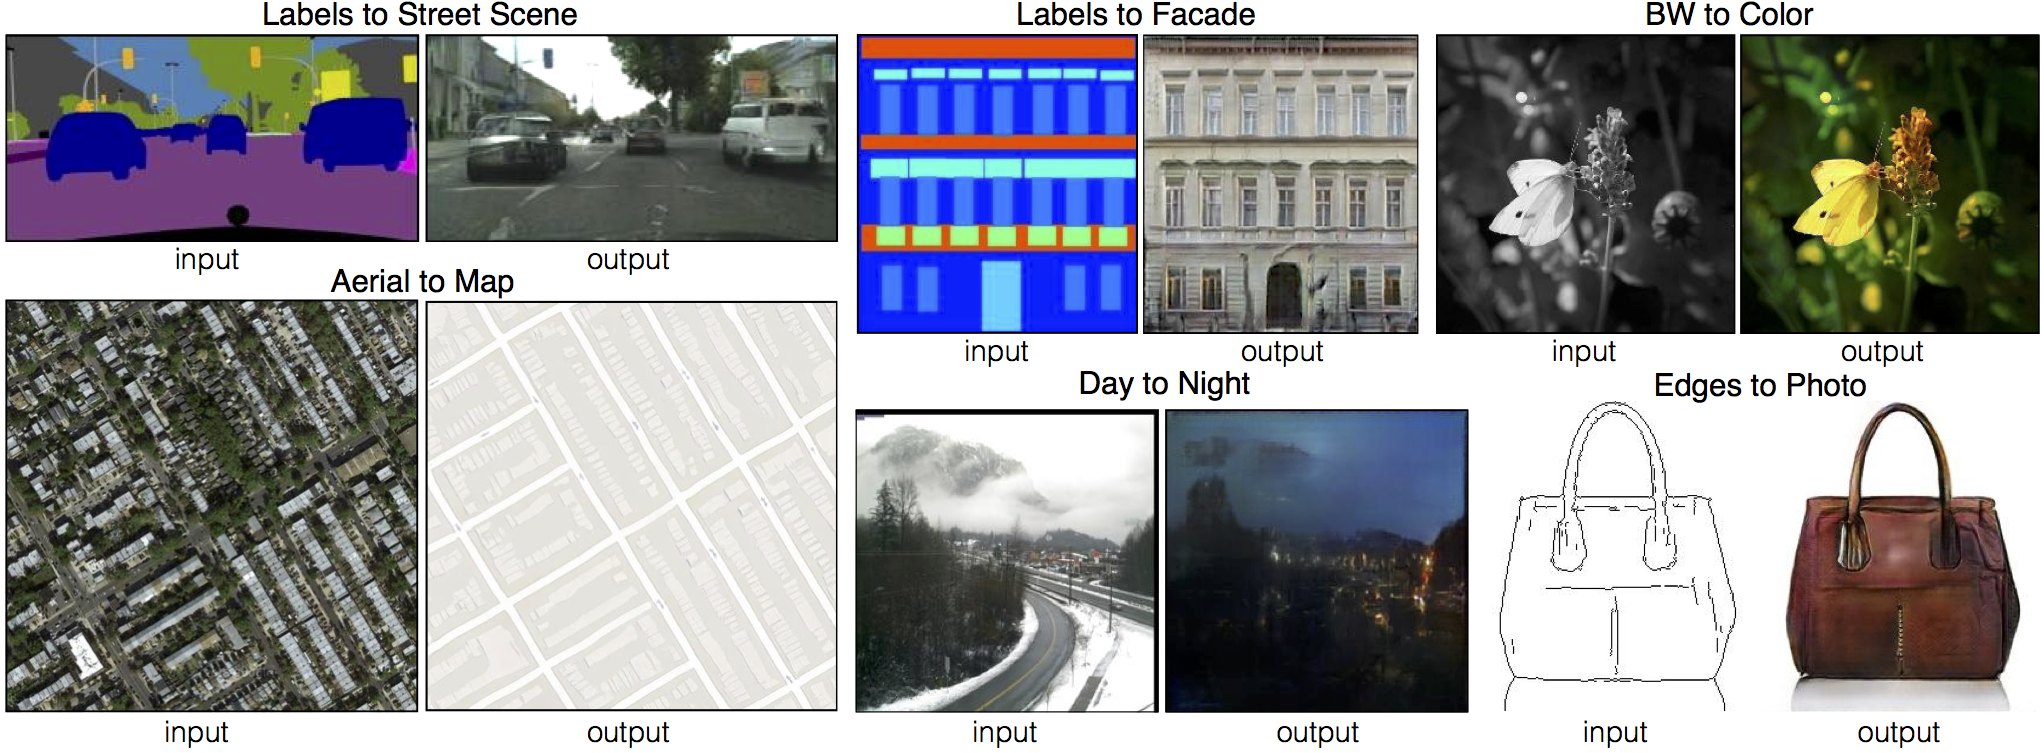
\includegraphics[width=0.7\columnwidth]{sections/figures/pix2pix.png}
    \caption{Pix2Pix image translation examples}
    \label{fig:my_label}
\end{figure}

Pix2Pix is a type of generative adversarial network used for image-to-image translation. Pix2Pix was presented by Phillip Isola in his 2016 paper \cite{DBLP:journals/corr/IsolaZZE16}. This architecture is used for many purposes that involve image-to-image translation as shown in the figure above. The author of End-to-End Image Colourisation decided to use this base architecture for image colourisation.




% For example, figure 2.5 shows the many possibilities Pix2Pix can achieve. For instance, it can be used to translate a sketch into a realistic photograph, Figure 2.5 also shows that a satellite image can be translated into something similar to google maps. Of course, the figure also demonstrates that image colourisation can be performed by translating black and white to its colour representation. The possibilities are quite endless as this architecture can be used to map nearly any arbitrary input to any arbitrary output.  

\subsubsection*{ChromaGAN}
\addcontentsline{toc}{subsubsection}{ChromaGAN}
The ChromaGAN is a conditional generative adversarial network proposed by the students from the University of Pompeu, Spain 2020 \cite{DBLP:journals/corr/abs-1907-09837}. Their proposal is primarily used for colourising grayscale images from semantic details engraved within the scene. Their method is an adaptation of \textbf{Let there be Color} since the generator of the architecture is inspired in the sense that it utilises a global feature extractor, but they decided to train this model in a GAN setting alongside a discriminator.

\begin{figure}[H]
    \centering
    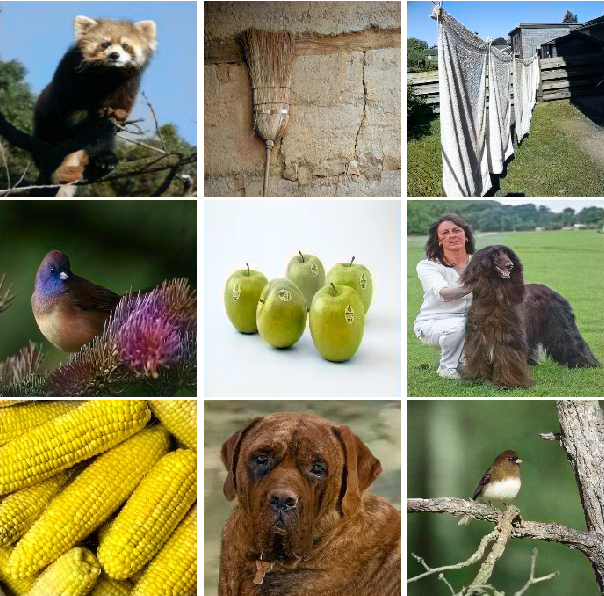
\includegraphics[width=0.5\columnwidth]{sections/figures/ChromaGAN.png}
    \caption{examples of ChromaGAN image colourisation}
    \label{fig:my_label}
\end{figure}




\subsection{Comparative literature review}


\begin{figure}[H]
    \centering
    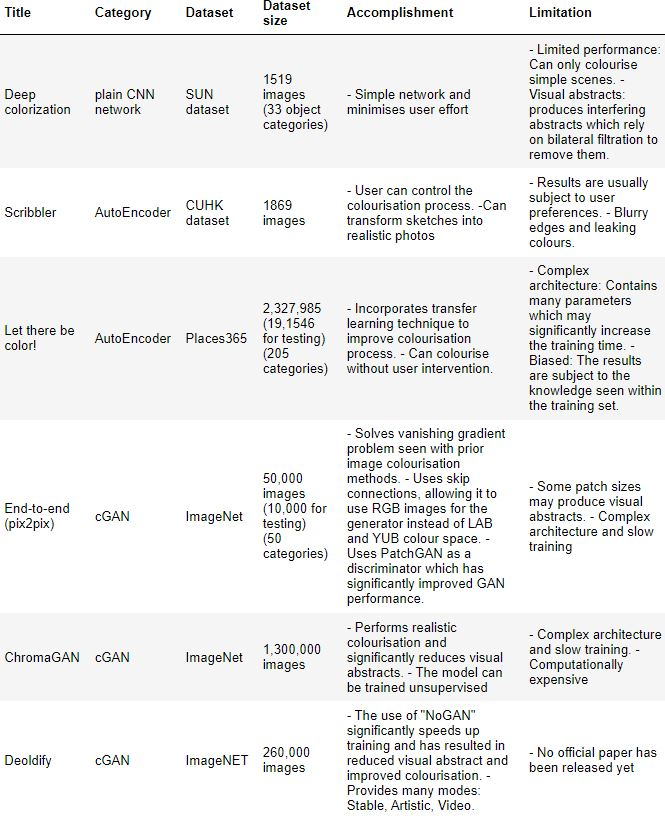
\includegraphics[scale=1,width=1\columnwidth]{sections/appendix/comparison.JPG}
    \caption{Advantages and disadvantages of each author's method}
    \label{fig:my_label}
\end{figure}

\subsection{RGB and LAB mapping}
In the task of image colourisation, the aim is to predict the colour channel of the given grayscale images. However in order to predict, a mapping between the grayscale pixel and the corrosponding coloured pixels is needed to be found defined colour space. 

\begin{figure}[H]
    \centering
    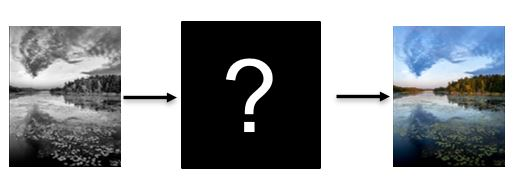
\includegraphics[width=0.7\columnwidth]{sections/figures/mapping.JPG}
    \caption{Image colourisation is a task of finding a mapping}
    \label{fig:my_label}
\end{figure}
As seen in the above figure, the task mainly involves finding a mapping such that a grayscale image (input) can be mapped to its corresponding coloured output. This mapping can be achieved by using a training set to discover all the related patterns used for mapping between grayscale and coloured. Here, the mapping can be achieved using two existing colour space representations: RGB and LAB.

% There exists a grey to colour mapping function \(F\) that can map the features contained at each pixel in a grayscale image \(L\) to learn the corresponding chrominance \(A*B*\) values from the image. The aim is to learn such a mapping function from the training set so that the conversion from grey to colour can be achieved using the function \(F\). 

\begin{figure}[H]
    \centering
    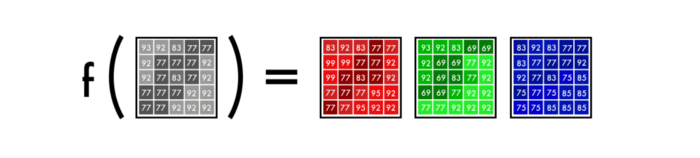
\includegraphics[width=0.6\columnwidth]{sections/figures/rgb.png}
    \caption{examples of ChromaGAN image colourisation \cite{wallner_2021}}
    \label{fig:my_label}
\end{figure}
One of the common representations is the RGB. This representation is widely used in electronic displays, such as computers, televisions, and cell phones. The RGB color model is an additive model in which red, green, and blue light are added together in different combinations to create a wide range of colors \cite{enwiki:1080368112}. For the task of colourisation, this representation will involve finding a mapping function to the three channels (as seen in the figure above). 


% \lipsum[1]
\begin{figure}[H]
    \centering
    
\includegraphics[width=0.6\columnwidth]{sections/figures/lab.png}
    \caption{examples of ChromaGAN image colourisation}
    \label{fig:my_label}
\end{figure}

There are other kinds of representations like LAB where L stands for luminance, and A and B for the colour spectra green–red and blue-yellow \cite{enwiki:1077444859}. Using the LAB colour channel in terms of image colourisation offers convenience as the L* channel represents the grayscale of the image and can be used as a conditional input. So while using the LAB representation, only 2 channels need to be mapped.


\pagebreak
\section{Similar Work}
\subsection{Human VS Objective evaluation of colorisation
performance}
Sean Mullery and Paul F. Whelan wrote a research investigation into evaluating image colourisation results using human and objective measures. Their research concerns more on whether the objective measures correlate with human opinion on images colourised using deep learning. They conducted a human evaluation test using Amazon mechanical Turk using 19 participants, and using their responses, they compared that against a dozen objective measures, to see if any of the objectives have a strong correlation with human opinion. 
The investigation concluded that the objective measures utilised in the colourisation literature did not correlate well with human opinion, with MS-SSIM showing the highest correlation, however, the correlation was too low to be considered an appropriate solution. They also reported on the behaviour of the observers, and noticed how most observers were tolerant to minor changes, but penalised heavily on medium to large changes \cite{https://doi.org/10.48550/arxiv.2204.05200}. 

\subsection{Image Colorization: A Survey and Dataset}
A comprehensive survey of various image colourisation methods was investigated by Saeed Anwar and Muhammad Tahir. This investigation was to address the need for a survey in the field of image colourisation. The survey involves the results of experiments on existing image colourisation methods. Here, they performed an extensive evaluation on several classes of architectures which are: Plain networks, user-guided networks, domain-specific networks, text-based networks, diverse colourisation networks, multi-path networks, and exemplar-based methods. Their investigation also discusses the many benefits and limitations of each existing colourisation method as well as mentions the same for datasets. Their report concluded that the current use of metrics used by many existing colourisation methods is inadequate to evaluate the colourisation, and also discovered how most image colourisation methods performed, such as how GAN-based methods delivered diverse colourisation whereas CNN-based methods tend to deliver sub-optimal results for complex scenes \cite{anwar2020ColorSurvey}. 

\subsection{A review of image colourisation}
A review of image colourisation was a report carried out by Bo Li, Yu-Kun Lai and Paul Rosin. Their paper discusses the history of image colourisation and goes on to mention automated-based image colourisation methods, with which they experimented. They perform an extensive evaluation of reference-based, user guidance-based and deep learning-based image colourisation methods and compare each method to see look for similarities and differences. Their report concluded that deep learning methods produced robust and meaningful results, however, were difficult to control. They also reported how no quantitative metrics exist to measure the quality of colourised results, mainly because how current metrics do not provide accurate measures for coloured images. They plan to investigate and develop a metric useful for coloured images as future work\cite{Li2019}.
\pagebreak
\section{Generative Neural Networks}
In deep learning there are neural networks and then there are generative neural networks. Here, I will only be mentioning the latter, so refer to Appendix B for information regarding Neural Networks.


\subsection{Auto encoder}
The autoencoder is a class of CNN, it is used to learn efficient coding of unlabeled data (unsupervised learning). Autoencoders attempt to learn representations (encoding) for a given set of data by decomposing the data into small bits of data (bottleneck). Then, the Autoencoder will use that representation to reconstruct (decoder) the original data \cite{IntroductionToAutoencoders}.
\begin{figure}[H]
    \centering
    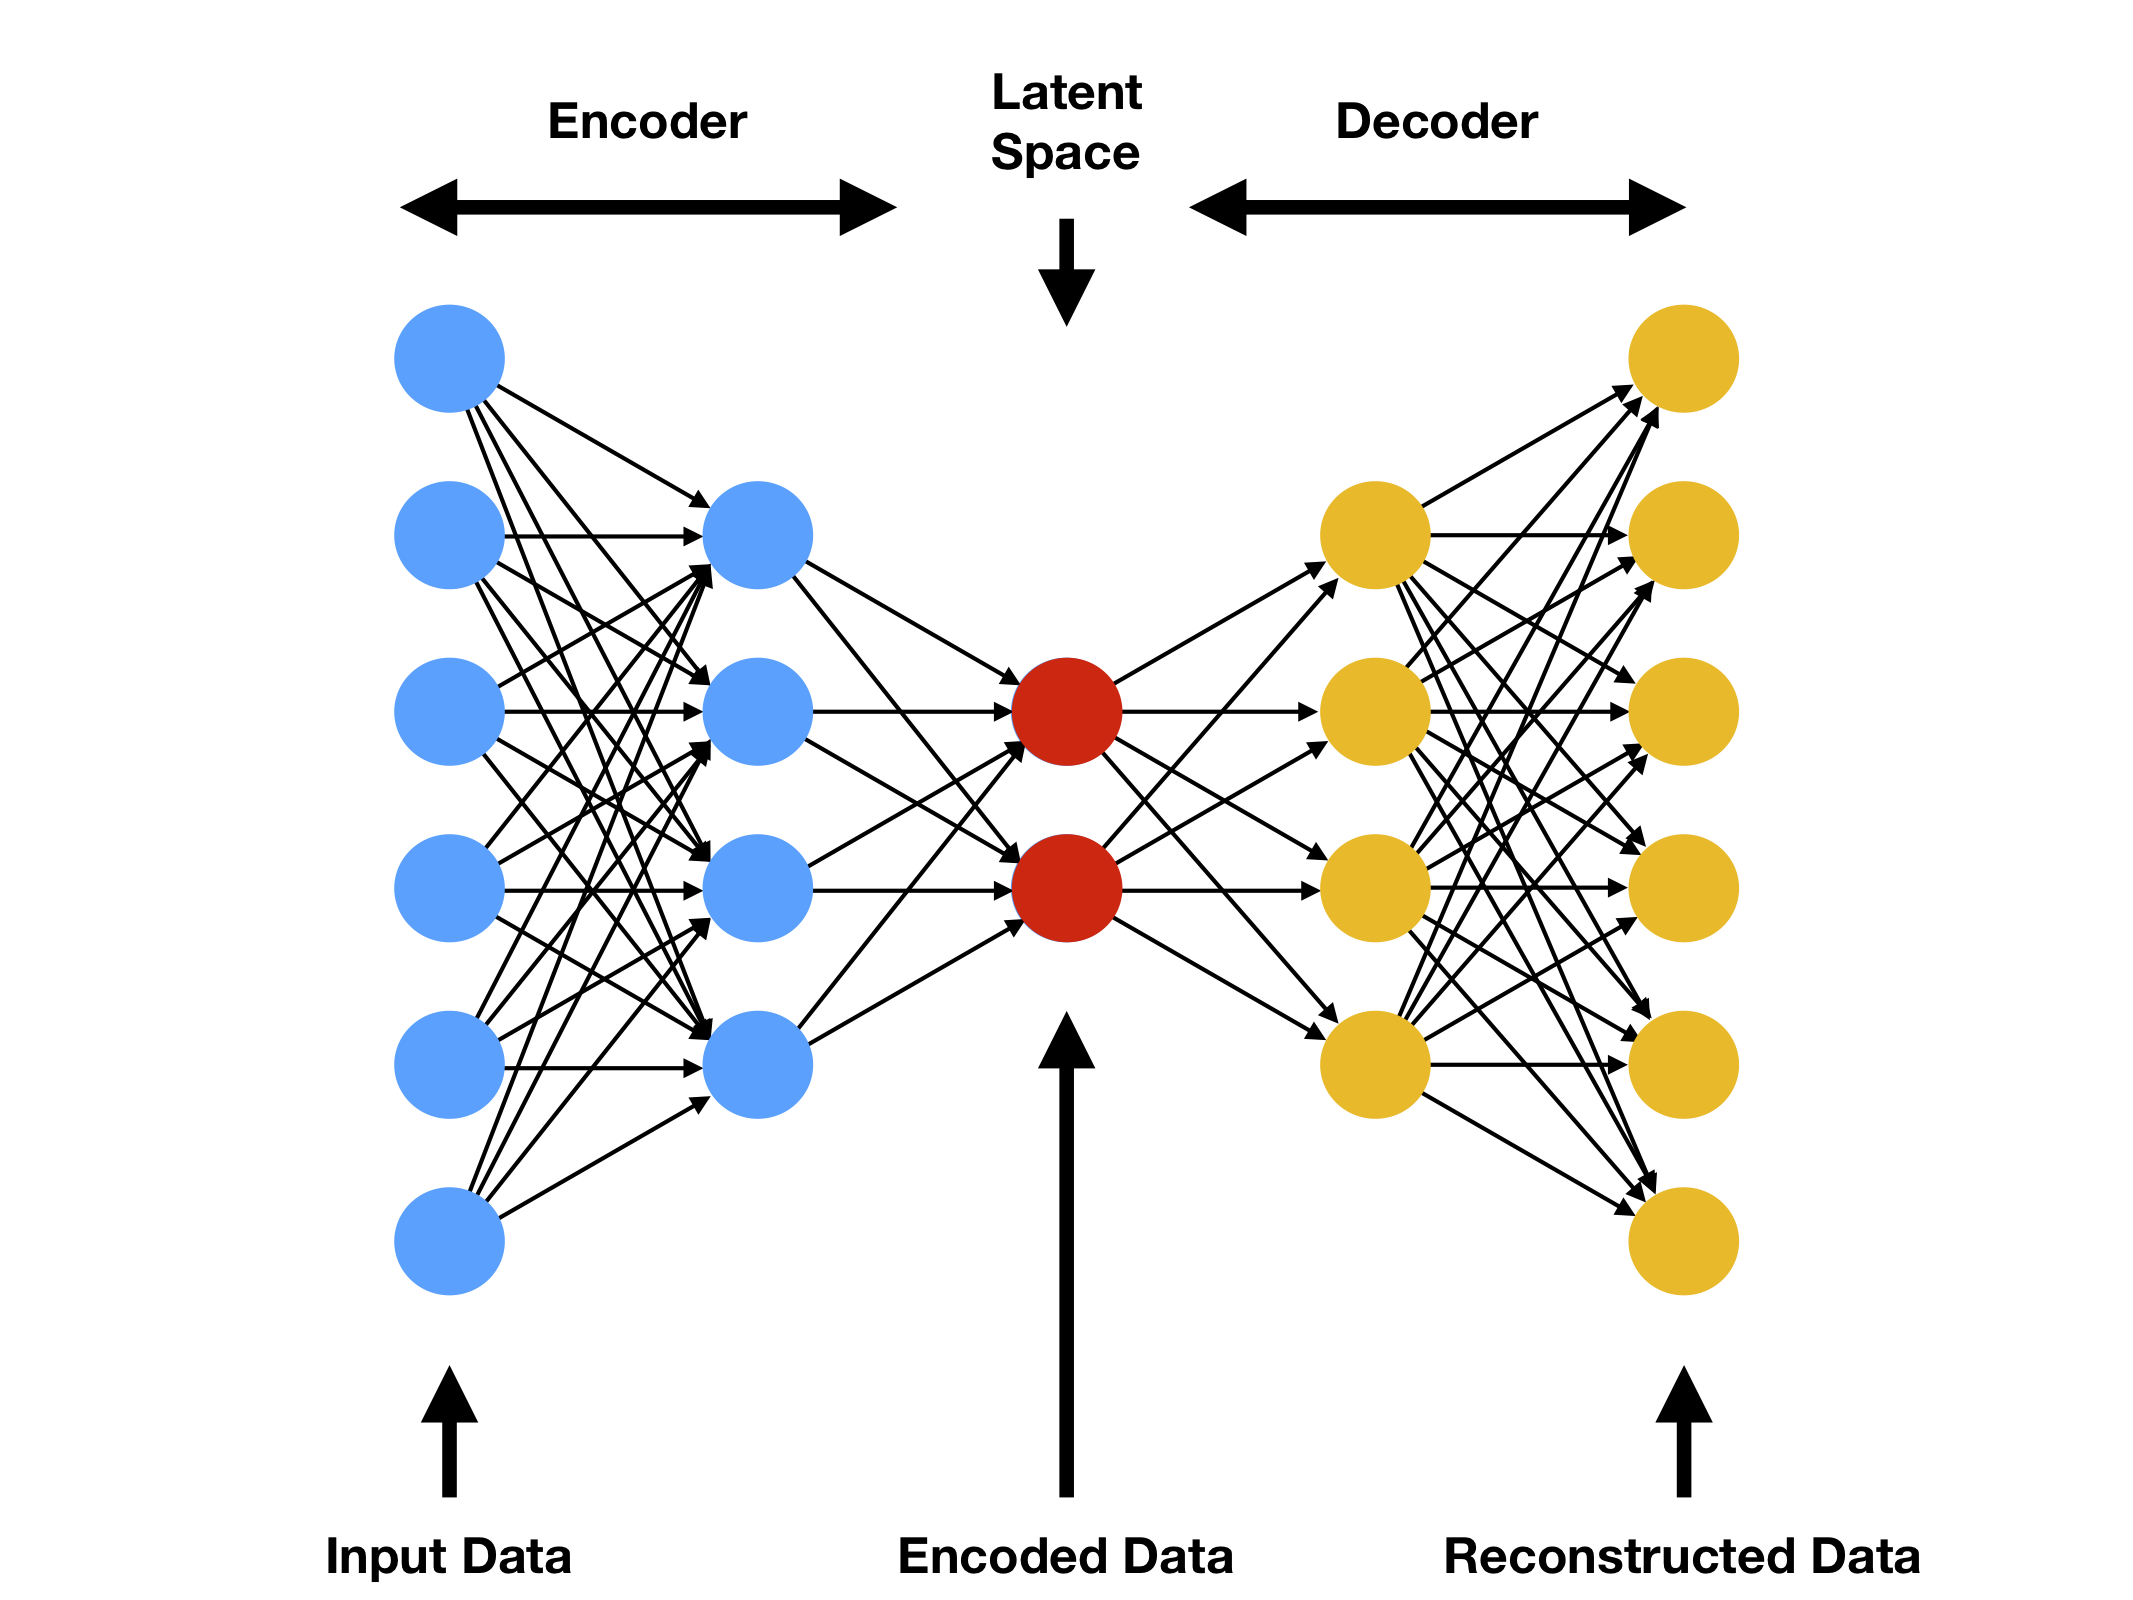
\includegraphics[width=0.6\columnwidth]{sections/figures/autoencoder_image.png}
    \caption{Example of an AutoEncoder model \cite{flores_2019}}
    \label{fig:my_label}
\end{figure}

\subsection{Generative Adversarial Networks}
A generative adversarial network (GAN) was introduced in 2014 by Goodfellow et al\cite{goodfellow2014generative}. The process of GAN involves a generator that generates an image, and its job is to fool the discriminator into thinking the generated image is real. As mentioned, the discriminator is used to determine whether the images presented by the generator are real or fake. If the image is deemed to be fake, the discriminator will pass feedback to the generator to suggest what the generator must do to improve its skill of making images that are indistinguishable from the real ones\cite{introToGanJasonBrownlee}. Both the generator and the discriminator are trained to outperform one another, eventually resulting in images that are increasingly realistic, making it impossible for the discriminator to tell the generated and the real images apart\cite{franoischollet2017learning}.
\begin{figure}[H]
    \centering
    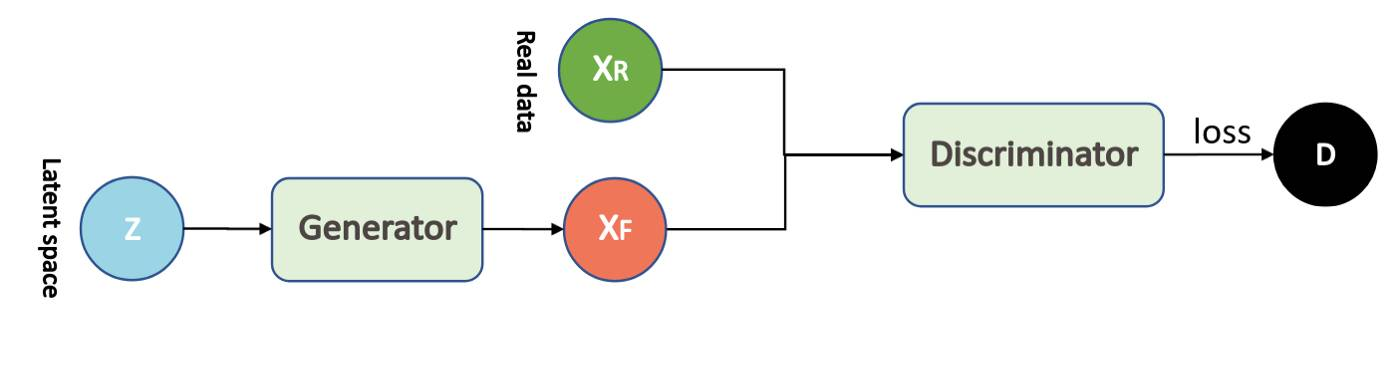
\includegraphics[width=0.7\columnwidth]{sections/figures/gan.JPG}
    \caption{Example of a gan model \cite{bagheri_2019}}
    \label{fig:my_label}
\end{figure}


\subsection{conditional GAN}
A cGan or conditional GAN is a generative adversarial network (GAN) that is conditioned on an additional input, typically an image. The cGan is different from a regular GAN in that it can generate images that are conditioned on a specific input, giving it the ability to generate images that are more realistic and diverse. The first cGan was developed by Mirza and Osindero in 2014. Some use cases for a cGan include generating realistic images, synthesizing images from text, and creating photo-realistic images\cite{frumkin_manipula_kachai_fehr_sewell}.
\begin{figure}[H]
    \centering
    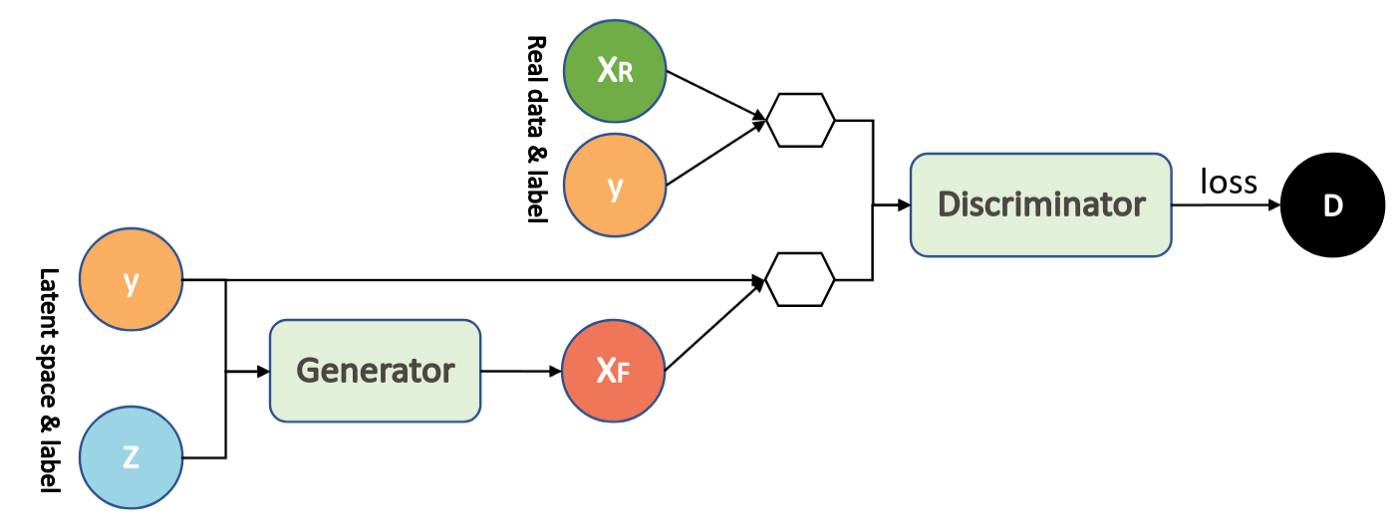
\includegraphics[width=0.7\columnwidth]{sections/figures/cgan.jpg}
    \caption{Example of a cGan model \cite{bagheri_2019}}
    \label{fig:my_label}
\end{figure}



\newpage
\section{Dataset}
In order for Machine learning models to understand how to perform various tasks, they'll first need to be trained using a sufficient amount of dataset. These datasets can be in various forms, such as numerical, categorical or time series, in my case I will be using numerical as it is a way of representing images. Datasets are often split up into 3 partitions: Training set which will be used to train the model; Validation set will be used to evaluate the model's performance during training; Testing set will be used to test the model's accuracy and performance after it has been trained. Since the models will perform image colourisation tasks, it'll need to be trained using an image dataset. Below are a few image datasets I have looked into that I can use to train the models:
\subsection{SUN dataset}
The Scene UNderstanding (SUN) dataset is a well-sampled dataset that contains about 130,519 annotated images spread over 899 categories \cite{sun}. The dataset is used by researchers specialising in the fields of computer vision, human perception, cognition, machine learning, and data science. Typically, the images in the dataset contain environmental scenes and everyday objects, which are all annotated with their corresponding category and name. The number of images in the SUN dataset is expanding constantly as new images are being annotated every day. In my case, this dataset provides a rich amount of images, which is already beyond the perfect amount needed to train the models.

\subsection{Places dataset}
The places dataset is an open-source large-scale image dataset used mainly for scene recognition in computer vision. The dataset contains 10 million scene photographs with annotations which makes it the largest existing scene-centric image dataset. This dataset is used in many applications within the world of computer vision, such as classification problems. The dataset contains a large number of natural images from a variety of places, including indoor and outdoor scenes. The dataset is divided into 365 categories, and each category contains a large number of images.\cite{Zhou1109}.


\subsection{Open Images Dataset}
The open images dataset is an open-source image dataset from Google. This dataset contains a significant amount of over 9 million images with annotations. It contains a total of 16 million boxes for 600 object classes on 1.9 million images, which makes it the largest existing dataset with object location annotation \cite{2020}. Like the SUN dataset, the open image dataset is expanding every single day, with each release adding millions of more annotated images. 
\newpage

\section{Requirements}
\subsection{Tensorflow}
\textbf{Tensorflow} is a powerful library used for \textbf{numerical tensor computation} and is primarily used for \textbf{creating and deploying large-scale Machine Learning models} and offers a plethora of tools. The library was first released for open source in 2015 by Google Brain Team and is now regarded as one of the\textbf{ most popular deep learning frameworks} to this day\cite{10.5555/3153997}. 


\subsection{Keras}
\textbf{Keras} is an open-source, deep-learning python library \textbf{developed by François Chollet in 2015} \cite{franoischollet2017learning}. The framework provides an interface used for defining and training any kind of deep learning model. However, for tensor computation, Keras has to rely on a \textbf{backend engine} such as TensorFlow which makes Keras a \textbf{high-level framework}. 


\subsection{Scikit-learn}
\textbf{Scikit-learn} is an open-source machine learning library used for the Python programming language and was \textbf{released in 2007 by French Data Scientist David Cournapeau}. The library \textbf{features several machine learning algorithms for classification, regression and clustering}. Additionally, the library offers utilities for applying transformations to data such as \textbf{Lab2RGB} and \textbf{RGB2LAB} (which will be used for this throughout my research project). NumPy is utilised for performing high-performance linear algebra and array operations \cite{enwiki:1065626908}.

\subsection{OpenCV}
\textbf{OpenCV} is an open-source multi-platform \textbf{computer vision library} that you can use to implement \textbf{object recognition, object tracking, 3D reconstruction, image matching, and image stitching}. It provides many powerful image processing and computer vision functions. It is \textbf{widely used by developers to develop computer vision} and machine learning applications\cite{enwiki:1072564905}.







    

\chapter{Research Methodology}
\section{The dataset}
Before the model can be trained, tested and validated, I will need to acquire a dataset. The dataset of choice was the "Places365" dataset \cite{DBLP:journals/corr/ZhouKLTO16}. This dataset contains images of places, specifically streets, buildings, mountains, glaciers, and trees, but also contains images of objects and entities such as cars, planes, people and animals. Additionally, the set contains about 105,000 256x256 images across 65 classes split 60:20:20 for training, testing and validation respectively. The dataset is primarily used for image classification and analysis, but in my case, the task will be image colourisation \cite{landscape}.
\section{Data Preprocessing}
To ensure the models can interpret the data for training and testing, the data should be prepossessed. In my case, a \textbf{tensorflow pipeline} was used. The pipeline takes images in batches and will apply numerous transformations. These transformations may involve:  

\begin{enumerate}
  \item Decoding batches of images into numerical tensors is achieved using OpenCV's "imread" function.
  \item Creating input and targets. Inputs and outputs can be either grayscale input and RGB output for methods that perform RGB mapping, or \(L*\) and \(A*B\) respectively for methods that perform LAB mapping.
  \item Resizing the images to a constant size of 256 x 256 to ensure consistent dimensionality.
  \item Scaling each pixel of the image down to a range of [0,1]. This is done by dividing the colour channels from the images by the value of 255 (as RGB ranges between 0-255)
  \item Augmentation transformations are applied. These augmentations involve random cropping, flipping and zooming. Note that augmentation isn't used when using the testing set pipeline.
\end{enumerate}
\begin{figure}[H]
    \centering
    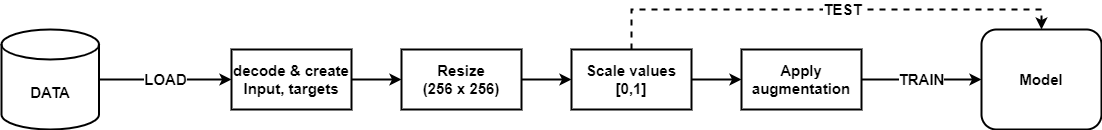
\includegraphics[width=1\columnwidth]{sections/figures/pipeline.png}
    \caption{Preprocessing pipeline}
    \label{fig:my_label}
\end{figure}






\pagebreak
\section{AutoEncoder method}
Here I've explored two AutoEncoder methods, Simple AutoEncoder and the Global AutoEncoder. 

Both models adopt the \(LAB\) colour space mapping since this colour space minimises the correlation between the three coordinate axes of the colour space.  




\subsection{Simple AutoEncoder}


\subsubsection*{Model Architecture}
\addcontentsline{toc}{subsubsection}{Model Architecture}
\begin{figure}[H]
    \centering
    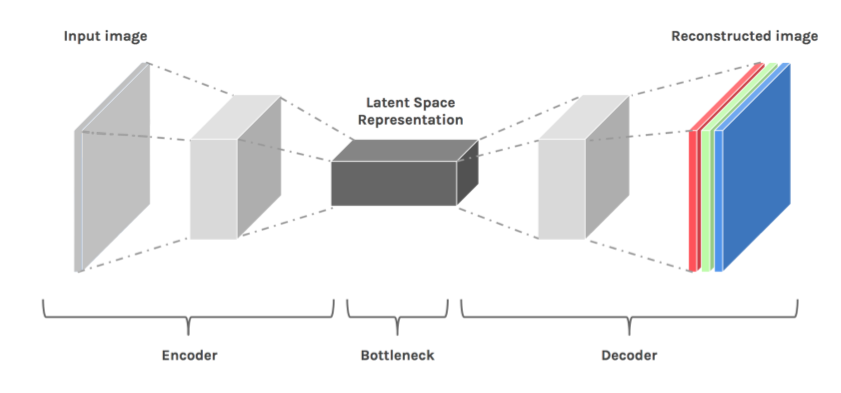
\includegraphics[width=0.7\columnwidth]{sections/figures/autoencoder.png}
    \caption{AutoEncoder architecture}
    \label{fig:my_label}
\end{figure}

The Simple AutoEncoder is regarded as the first method I experimented with during my research into image colourisation. The Architecture being used is based on \cite{IizukaSIGGRAPH2016} but without the Global Feature Extractor. For the sake of this report, this AutoEncoder will be referred to as \textbf{Simple AutoEncoder}.

This architecture is considered simple as out of all the methods I have experimented with, this model uses the fewest amount of parameters.

The basic anatomy of this AutoEncoder involves three distinct parts: the Encoder unit, Bottleneck \& the Decoder unit.

\subsubsection*{Encoder unit}
\addcontentsline{toc}{subsubsection}{Encoder unit}

The low-level features are encapsulated as part of the encoder. The encoder extracts features from the input image and comprises 10 convolution layers, each consisting of 3x3 kernels. The input of the encoder is the grayscale image, which represents H x W x 1, where H and W refer to the image's height and width. The result of the encoder represents H/8 x W/8 x 512. Setting each layer's padding to "same" helps to preserve the original image size. Strides are used at each convolution layer, this helps to reduce the output of the image by 50\%. Ultimately, the output image is decomposed into a latent space representation.

\subsubsection*{Bottleneck unit}
\addcontentsline{toc}{subsubsection}{Bottleneck unit}
The bottleneck unit of the autoencoder is the unit in the middle of the network that has the smallest number of neurons. This unit provides the lowest level of abstraction for the input data and forces the autoencoder to learn to compress the input data into a lower-dimensional representation.

\subsubsection*{Decoder unit}
\addcontentsline{toc}{subsubsection}{Decoder unit}


The decoder takes the bottleneck output as input and uses it to estimate the colours of the image. During this process, several upsample layers are used to increase the spatial H x W of the feature maps, using the UpSample2D. The produced output is the roughly estimated A*B* channels, with the H x W x 2 volume representation. The output of the decoder is then concatenated with the input grayscale channel to form the full L*A*B* image, which is then converted to RGB representation.
\pagebreak
\subsection{Global AutoEncoder method}

\subsubsection*{Model Architecture}
\addcontentsline{toc}{subsubsection}{Model Architecture}

\begin{figure}[H]
    \centering
    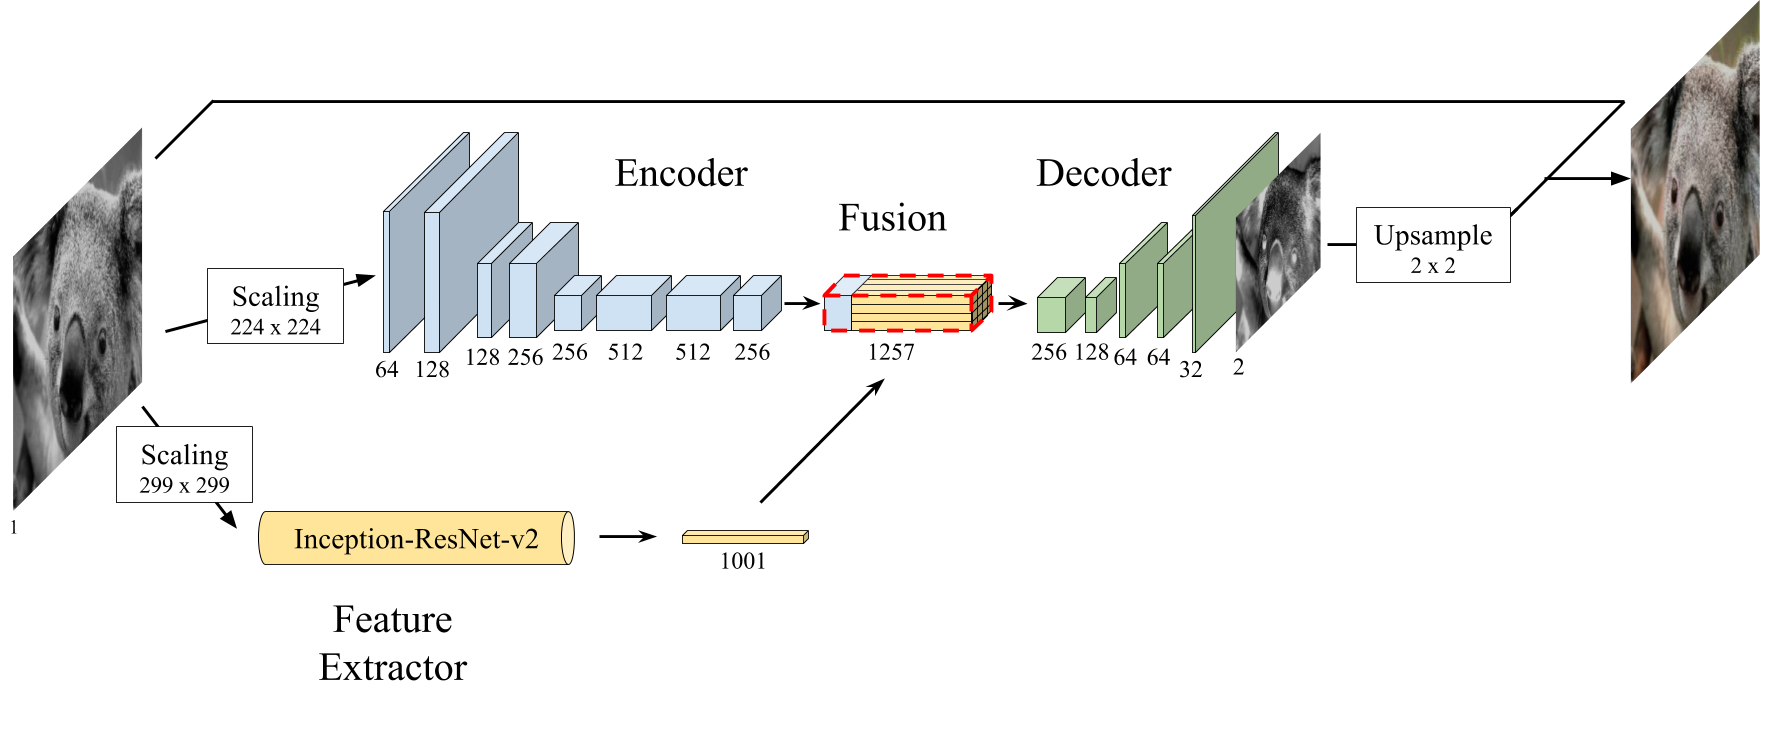
\includegraphics[width=1\columnwidth]{sections/figures/model.png}
    \caption{Deep Koalarization  architecture}
    \label{fig:my_label}
\end{figure}

The base architecture used for the image colourisation model is a form of an autoencoder and was developed by Federico Baldassarre, Diego Gonzalez-Morin and Lucas Rodes-Guirao \cite{deepkoal2017}. Their model was based on the authors of \cite{IizukaSIGGRAPH2016} (as seen in Figure 11).

\begin{figure}[H]
    \centering
    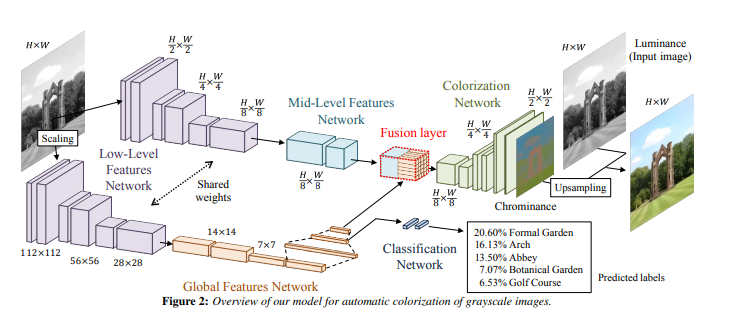
\includegraphics[width=0.8\columnwidth]{sections/figures/different_model.PNG}
    \caption{Let there be color architecture}
    \label{fig:my_label}
\end{figure}

\cite{deepkoal2017} (figure 3.3) use a pre-trained model (Inception-Resnet-V2) as a global feature extractor, whereas \cite{IizukaSIGGRAPH2016} (figure 3.4) use their own trained model for this purpose. The use of a pre-trained model for the global feature extractor eliminates the need to train a separate model, as the inception-ResNet-v2 has been trained over 1000 classes of images.

This model consists of four parts: the encoder, global feature extractor, fusion layer, and decoder. The encoder takes in the L channel (grayscale) and extracts low-level features. The input is also fed into a global feature extractor (GFE) which extracts global features. The fusion layer then combines the outputs of GFE and encoder. The fusion layer's output is then fed into the decoder, which does the colourisation task by mapping outputs to their corresponding colour channels.
 
The base AutoEncoder (without the global feature extractor) architecture used is identical to the previous simple AutoEncoder mentioned previous section, hence I will not go over the implementation again for this method, but rather will go over the highlighted differences. For the sake of this report, I will be referring to this architecture as \textbf{Global AutoEncoder}.

\subsubsection*{Global feature extractor}
\addcontentsline{toc}{subsubsection}{Global feature extractor}


The global feature extractor helps to identify and extract global features from the image and outputs a class distribution. The model is a pre-trained inception-resnet. It takes as input a grayscale image input which is upscaled to H x W of 299 x 299 respectively. The output of GFE will result in the image representing a 1000-dimensional class distribution vector. The point of the GFE is to indicate the class of the image from the given input so that it can help identify relevant colours. For instance, if the GFE identified the image as being an indoor room consisting of furniture, the GFE will mitigate the encoder from being biased, so that it will add appropriate colours for furniture, rather than sky or grass colours. 

\subsubsection*{Fusion Layer}
\addcontentsline{toc}{subsubsection}{Fusion Layer}



The fusion layer combines the output of the GFE (a 256 dimensional vector) and the encoder. The use of the fusion layer results with a H/8 x W/8 x 256 layer. This effectively merges the information gathered from the GFE and the encoder into one layer. The formula for fusion can be seen as:
\begin{equation}
y_{u,v}^{fusion} = \sigma \left ( b + W \begin{bmatrix}y^{global} \\y_{u,v}^{mid}  \end{bmatrix} \right )
\end{equation}

Where \(y_{u,v}^{fusion}\) is the fusion of features \(u,v\). Where \(y^{global} \) is the global feature vector and \(y_{u,v}^{mid} \) is the mid level feature at (\(u,v\)). \(W\) is the weights and \(B\) is the bias. Both, \(W\) and \(B\) are trainable variables. 


\pagebreak
\section{Conditional GAN method}
I have experimented with two different types of conditional GANs, ChromaGAN and Pix2Pix, to see if they perform better than the AutoEncoder methods that were discussed earlier.

\subsection{Pix2Pix GAN}
\begin{figure}[H]
    \centering
    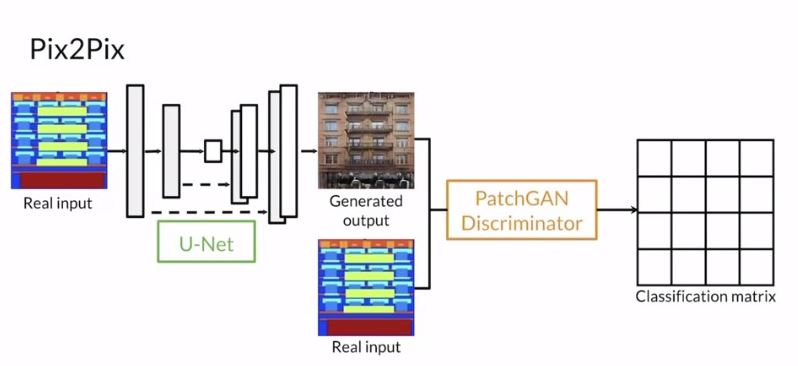
\includegraphics[width=1\columnwidth]{sections/figures/pix2pix_architecture.JPG}
    \caption{Pix2Pix Architecture}
    \label{fig:my_label}
\end{figure}

Pix2Pix is a category of cGAN and is used for image to image translation. This network not only can learn the mapping from an input image to an output image but also learns the loss function to train this mapping.

Pix2pix was developed as a more sophisticated approach to image-to-image translation, compared to the basic CNN method which simply minimizes the Euclidean distance between the predicted and ground truth pixels. However, it was seen that this method would result in a blurry output, as the Euclidean distance is minimized by averaging up all the outputs, causing the blurring effect.

In brief, the architecture works by learning a loss function that tries to classify the output image as being either real or fake, while simultaneously training a generative model to minimise this loss. Blurry images will not be tolerated as they will easily look fake.

\subsubsection*{U-NET Architecture (Generator)}
\addcontentsline{toc}{subsubsection}{U-NET Architecture (Generator)}

\begin{figure}[H]
    \centering
    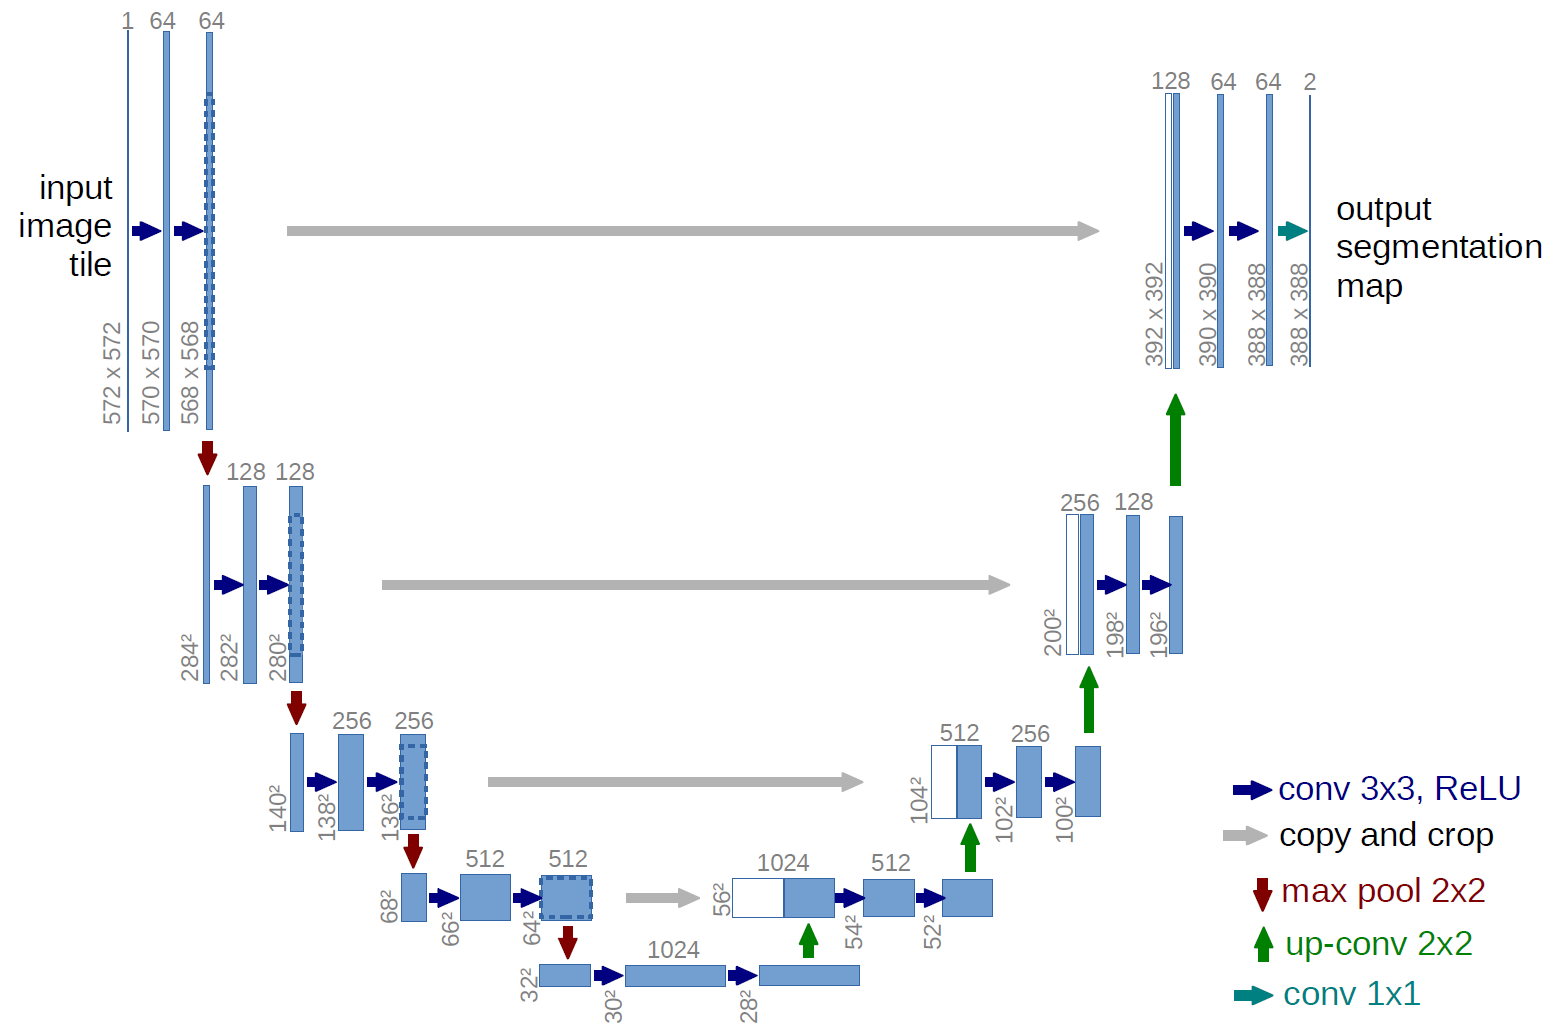
\includegraphics[width=0.7\columnwidth]{sections/figures/U-net.JPG}
    \caption{U-NET model \cite{RFB15a}}
    \label{fig:my_label}
\end{figure}

The most important aspect of the cGAN is the generator, as this is responsible for generating the coloured output. As discussed earlier, Pix2Pix can only work if the output image is not blurry, and having such blurry images will only help the discriminator in identifying the generated images. The AutoEncoder method I discussed earlier uses an encoder-decoder network. In these networks, the input image is progressively decomposed through the layers until it reaches a bottleneck, and from there the process is reversed. However, since the information is constantly being decomposed, information that helped retain the structures of the input image is risked being lost.

To mitigate this issue, the generator can utilise skip connections which creates the shape of a "U-Net". This architecture adds skip connections between each \(ith\) and the \(n - i\), where \(n\) represents the number of layers in the network. Using skip connection help pass information between the encoder and the decoder, information that involves the underlining structure, which helps mitigate the blurry effect, and also why this architecture can use the RGB mapping, previously sought to produce blurry images an AutoEncoder. 

\subsubsection*{PatchGan Architecture (Discriminator)}
\addcontentsline{toc}{subsubsection}{PatchGan Architecture (Discriminator)}
\begin{figure}[H]
    \centering
    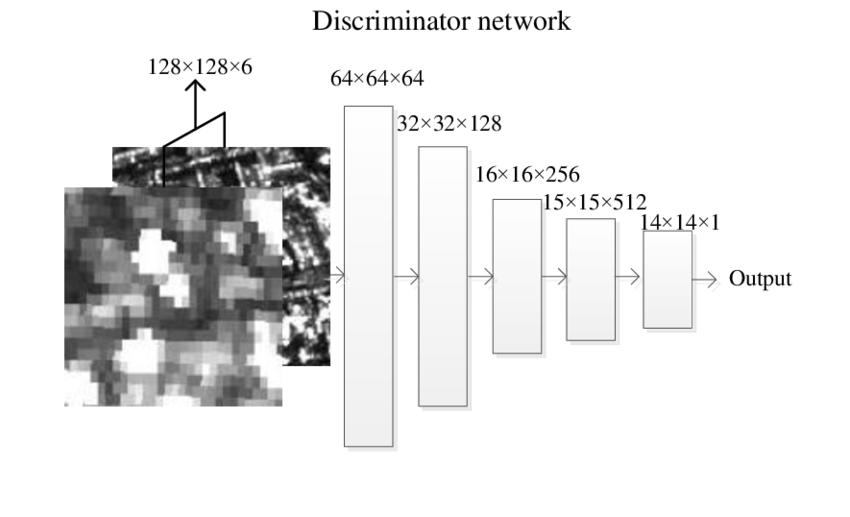
\includegraphics[width=0.7\columnwidth]{sections/figures/PatchGAN.png}
    \caption{PatchGAN model \cite{ao_2018}}
    \label{fig:my_label}
\end{figure}
The architecture of the discriminator used in Pix2Pix is based on the Markovian discriminator architecture, also known as patchGAN \cite{etal_2018}. PatchGAN is used for binary classification. This discriminator is used to address blurry images when using L1 loss and L2 loss on high frequency, however, it turned out that having L1 loss switched to low frequency helped mitigate this issue. The way this architecture works is by dividing the input image into \(N x N\) patches and then identifying each patch of the image as either real or fake. 

The size of the \(N\) patch was noted to influence the output of the image. Using smaller patches was reported to speed up training time, and the results often looked high quality. 
The discriminator is created using convolutional layers and LeakyRelU was used as this was reported to help solve the vanishing gradient problem \cite{brownlee_2020}. 





\newpage
\subsection{ChromaGAN}

\begin{figure}[H]
    \centering
    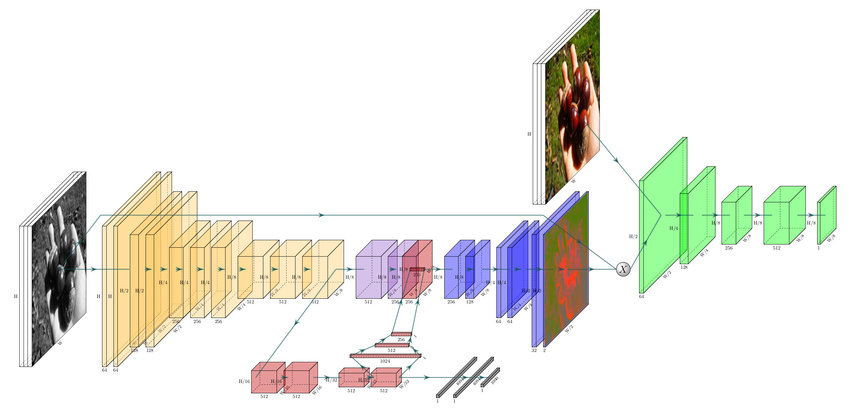
\includegraphics[width=1\columnwidth]{sections/figures/ChromaGAN_architecture.png}
    \caption{ChromaGAN Architecture}
    \label{fig:my_label}
\end{figure}

The ChromaGAN architecture is a conditional GAN. This architecture was developed by researchers from the University Pompeu Fabra \cite{DBLP:journals/corr/abs-1907-09837}. This architecture was developed for the purpose of colourisation of grayscale images. 

The difference between this architecture and the Pix2Pix method is the generator. ChromaGAN uses an AutoEncoder, which is similar to the global AutoEncoder discussed earlier. It performs LAB mapping and utilises a pre-trained global feature extractor, which is used to learn the class distribution vector. The distribution vector enables the information about the probability distribution within the semantic information contained within input \(L\), and this helps improve the colourisation performance without the need for a labelled dataset.




\subsubsection*{Generator Architecture}
\addcontentsline{toc}{subsubsection}{Generator Architecture}

The generator of the ChromaGAN is a network divided into two subnetworks: the AutoEncoder (yellow, purple and blue parts shown in figure 3.7) and the global feature extractor (red parts shown in figure 3.7). Here, I will be denoting both networks as \(G^1\) and  \(G^2\). Both \(G^1\) and \(G^2\) take as input a \(H x W\) image. \(G^1\) outputs chrominance information represented as \((a,b) = G^1(L)\), and \(G^2\) outputs the class distribution vector \(y = G^2(L)\). \(G^2\) can only take in the input of channel size of 3, so the input image requires broadcasting, which involves concatenating the input image three times \([L,L,L]\). \(G^2\) uses the pre-trained VGG-16 weights, but they are kept unfrozen during the process of training.

The encoder output of \(G^1\) (represented in orange in figure 3.7) is then fused with the class distribution output produced from \(G^2\). The fused output is then fed as input into the last stage of \(G^1\), which is the decoder. The decoder will process this information through six modules of CNN layers with ReLu activation functions, along with two upsampling layers between them. The produced output is then concatenated with the input to form the full coloured image which will then be used against the adversary.

\subsubsection*{Discriminator Architecture}
\addcontentsline{toc}{subsubsection}{Discriminator Architecture}

The discriminator of the ChromoGAN is the patchGAN. The patchGAN discriminator has already been discussed as pix2pix also uses the same discriminator. To be brief, it is noted that this architecture exceeds when working when capturing low-frequency structure of the input image, however, fails when working at high frequency. This process involves dividing the \(H x W\) input into patches and then classifies each individual patch of the image. The size of the patch was noted to influence the performance, as using smaller patches helped speed up performance and increase the quality of the input image produced by the generator.




\pagebreak
\section{Training and evaluation}
 Out of the \textbf{105,000} samples from the Places dataset, \textbf{84,000} was reserved for training whilst \textbf{21,000} was used for\textbf{ testing and evaluation}.

All models were trained using \textbf{Slurm Facility} which is an workload manager for scheduling jobs for large scale cluster. \cite{enwiki:1078654743}. The university provided me this service, and it allowed me to train the models practically for free.

Unfortunately, I could not leverage the time I had for optimisation. As a compromise, I will be sticking to the author's chosen hyper-parameter and will be performing quantitative testing using evaluation metrics. In the interim, I have performed tuning using a smaller dataset, please refer to Appendix B for this. 

\textbf{Nvidia Cuda} Toolkit with\textbf{ Nvidia Tesla M10} were used to enable GPU acceleration for faster training. The training time between each method was different, as some methods took 1 day to train whereas others took up to 4 days. 


\subsection{Objective functions}
The objective function is a key component in deep learning because it provides a way to find the optimal solution \cite{kronovet_2017}. The objectives may involve minimising or maximising a value. This value may represent an error used to quantify the distance between the predictions and the targets. The algorithm will continuously configure the model's parameters to minimise this error. Therefore, the use of an objective is essential in deep learning.

Since I have researched the 4 methods discussed throughout this section, it's known that each method has its own unique objective function.

\subsubsection*{AutoEncoder Objective function}
\addcontentsline{toc}{subsubsection}{AutoEncoder Objective function}
Both AutoEncoder methods discussed so far use the same objective function. This objective function can be defined as computing the distance between the estimated output and the target output. A Mean Square Error loss function is used to quantify the error between the estimated pixel and the target pixel. The objective function can be denoted as the following formula:
\begin{equation}
C(X,\theta ) = \frac{1}{2HW}\sum_{k \in (a,b)}^{}\sum_{i=1}^{H}\sum_{j=1}^{W}||X_{k_{i,j}} - \hat{X}_{k_{i,j}} ||^2
\end{equation}
Where \(\theta\) represents the parameters of the model, \( X_{k_{i,j}} \) and \( \hat{X}_{k_{i,j}} \) denote the \(i,jth\) pixel value of the \(kth\) channel value contained in the target and reconstructed predicted image respectively. The \(||.||^2\) is the euclidean distance used to compute the difference between \( X_{k_{i,j}} \) and \( \hat{X}_{k_{i,j}} \). 
% 
Both methods employ the same optimiser which is Adam to minimise this objective. This optimiser is preferred because it can handle sparse gradients on noisy problems such as natural language and computer vision \cite{brownlee_2021}. 
Both methods have an initial learning rate set at 0.0001.



\subsubsection*{Pix2Pix Objective function}
\addcontentsline{toc}{subsubsection}{Pix2Pix Objective function}
The objective function for Pix2Pix is unique compared to the AutoEncoder methods mentioned above, as both entities of the cGAN, the generator and the discriminator are competing against one another over the same objective. The anatomy of how Pix2Pix performs is through an objective function expressed below:
$$
\begin{aligned}
\arg \min _{G} \max _{D} \mathcal{L}_{c G A N}(G, D)+\lambda \mathcal{L}_{L 1}(G)
\end{aligned}
$$
Where \(G\) represents the Generator that is tasked to minimise the objective against the discriminator \(D\) which tries to maximise it. In addition to the objective, a \(\mathcal{L}_{L 1}(G)\) cost is added, and can be expressed as:

$$
\mathcal{L}_{L 1}(G)=\mathbb{E}_{x, y, z}\left[\|y-G(x, z)\|_{1}\right]
$$
The \(L1\) distance is used instead of the \(L2\) as it was discussed earlier that using \(L1\) encouraged less blurring in images.

The Adam optimiser is used to minimise this objective with the learning rate set at \(2e-4\) and the momentum parameters set at \(\beta_1 = 0.5\) and \(\beta_2 = 0.999\).



\subsubsection*{ChromaGAN Objective function}
\addcontentsline{toc}{subsubsection}{ChromaGAN Objective function}
The objective of the ChromaGAN is similar to Pix2Pix, both generator and discriminator are continuously competing against one another. The objective is defined by the following formula:
\begin{equation}
\arg \min _{G} \max _{D} \mathcal{L}_{c G A N}(G, D)
\end{equation}
However, the difference lies within the \(\mathcal{L}_{c G A N}(G, D)\) objective function:
\begin{equation}
\mathcal{L}_{c G A N}(G, D)=\mathcal{L}_{\mathrm{e}}\left(\mathcal{G}_{\theta_{1}}^{1}\right)+\lambda_{\mathrm{g}} \mathcal{L}_{\mathrm{g}}\left(\mathcal{G}_{\theta_{1}}^{1}, D_{w}\right)+\lambda_{\mathrm{s}} \mathcal{L}_{\mathrm{s}}\left(\mathcal{G}_{\theta_{2}}^{2}\right)
\end{equation}

The first term in the equation, $\mathcal{L}_{\mathrm{e}}\left(\mathcal{G}_{\theta_{1}}^{1}\right)$, is the color error loss of the encoder-decoder part of the generator. The second term, $\lambda_{\mathrm{s}} \mathcal{L}_{\mathrm{s}}\left(\mathcal{G}_{\theta_{2}}^{2}\right)$, is the class distribution loss produced by the VGG-16 model.

This objective is minimised using the Adam optimiser which has a set learning rate of 2e-5 and has the momentum parameters set at \(\beta_1 = 0.5\) and \(\beta_2 = 0.999\).


\pagebreak
\subsection{Evaluation Metrics}
% Due to the black box nature of the Deep Learning models, deploying them requires extensive verification and testing to gain insights into the decision-making process \cite{electronics10050593}. Without this, determining the success of the model's performance on unseen data, and identifying whether the algorithms have overfitted the training data will be difficult. Hence, the need for evaluation metrics is essential to help verify the model's performance on unseen data. This is also known as generalisation; the goal of every deep learning model is to have good generalisation \cite{enwiki:1073306062}.

% However, finding a quantitative metric to evaluate the performance of all discussed methods is a challenging task, as not all methods could rely on an agreed method of evaluation. Fortunately, the authors of the methods all used common methods: PSNR, SSIM and Perception test.
Due to the black box nature of Deep Learning models, extensive testing and validation is require to gain insight into the decision-making process \cite{electronics10050593}. This can be done using various techniques. Here, I will be using PSNR, SSIM and Naturalness study to conduct me evaluation.

\subsubsection*{PSNR score}
\addcontentsline{toc}{subsubsection}{PSNR score}
The Peak Signal-to-Noise Ratio (PSNR) is an objective metrics used to calculate the ratio in decibels between two images. This ratio is used to measure the quality between the target image and the original image. The ratio is used to indicate the quality of the output image; the higher the ratio, the better the quality of the output image. It's essentially another way of estimating the similarities between the colourised image and the ground truth \cite{Chauhan2018}. The formula for calculating the PSNR score is as follows:
\begin{equation}
\begin{gathered}
P S N R=10 \log _{10}\left(\frac{M A X_{l}^{2}}{M S E}\right) \\
M S E=\frac{1}{m n} \sum_{i=0}^{m-1} \sum_{j=0}^{n-1}[I(i, j)-K(i, j)]^{2} 
\end{gathered}
\cite{anon_2014}
\end{equation}
Where \(M A X_{l}\) represents the maximum pixel value of the image, whereas the \(M S E\) is used to measure the difference between the original and target image.


\subsubsection*{SSIM score}
\addcontentsline{toc}{subsubsection}{SSIM score}
SSIM (structural similarity index measure) is another objective metric used for quantifying the differences or similarity between two images. This metric is meant to serve as an alternative to the PSNR score, and unlike the PSNR score, the SSIM score can capture visible structure of the image \cite{1284395}.

The SSIM index is calculated as:
\begin{equation}
\operatorname{SSIM}(f, g)=l(f, g) c(f, g) s(f, g)
\end{equation}
where
\begin{equation}
\left\{\begin{array}{l}
l(f, g)=\frac{2 \mu_{f} \mu_{g}+C_{1}}{\mu_{f}^{2}+\mu_{g}^{2}+C_{1}} \\
c(f, g)=\frac{2 \sigma_{f} \sigma_{g}+C_{2}}{\sigma_{f}^{2}+\sigma_{g}^{2}+C_{2}} \\
s(f, g)=\frac{\sigma_{f g}+C_{3}}{\sigma_{f} \sigma_{g}+C_{3}}
\end{array}\right.
\cite{5596999}
\end{equation}

The first term is the luminance comparison of the two images. The second term is the contrast comparison and the last term is used for structural comparison of the two images. A SSIM of 1 means both images are the same, whereas a high SSIM denotes a high similarity and a low SSIM means there's little to nothing in common between the two images. 



\pagebreak
\subsubsection*{Naturalness study}
\addcontentsline{toc}{subsubsection}{Naturalness study}
The naturalness study is another form of quantitative evaluation, however, unlike previous objective metrics (PSNR & SSIM), this method relies on human opinion. The way the natural study works is by providing a naturalness perception test to volunteers. Each volunteer was given instructions (see figure 3.8 below) and their job is to agree or disagree on whether the colours of the image looked natural or not.

\begin{figure}[H]
    \centering
    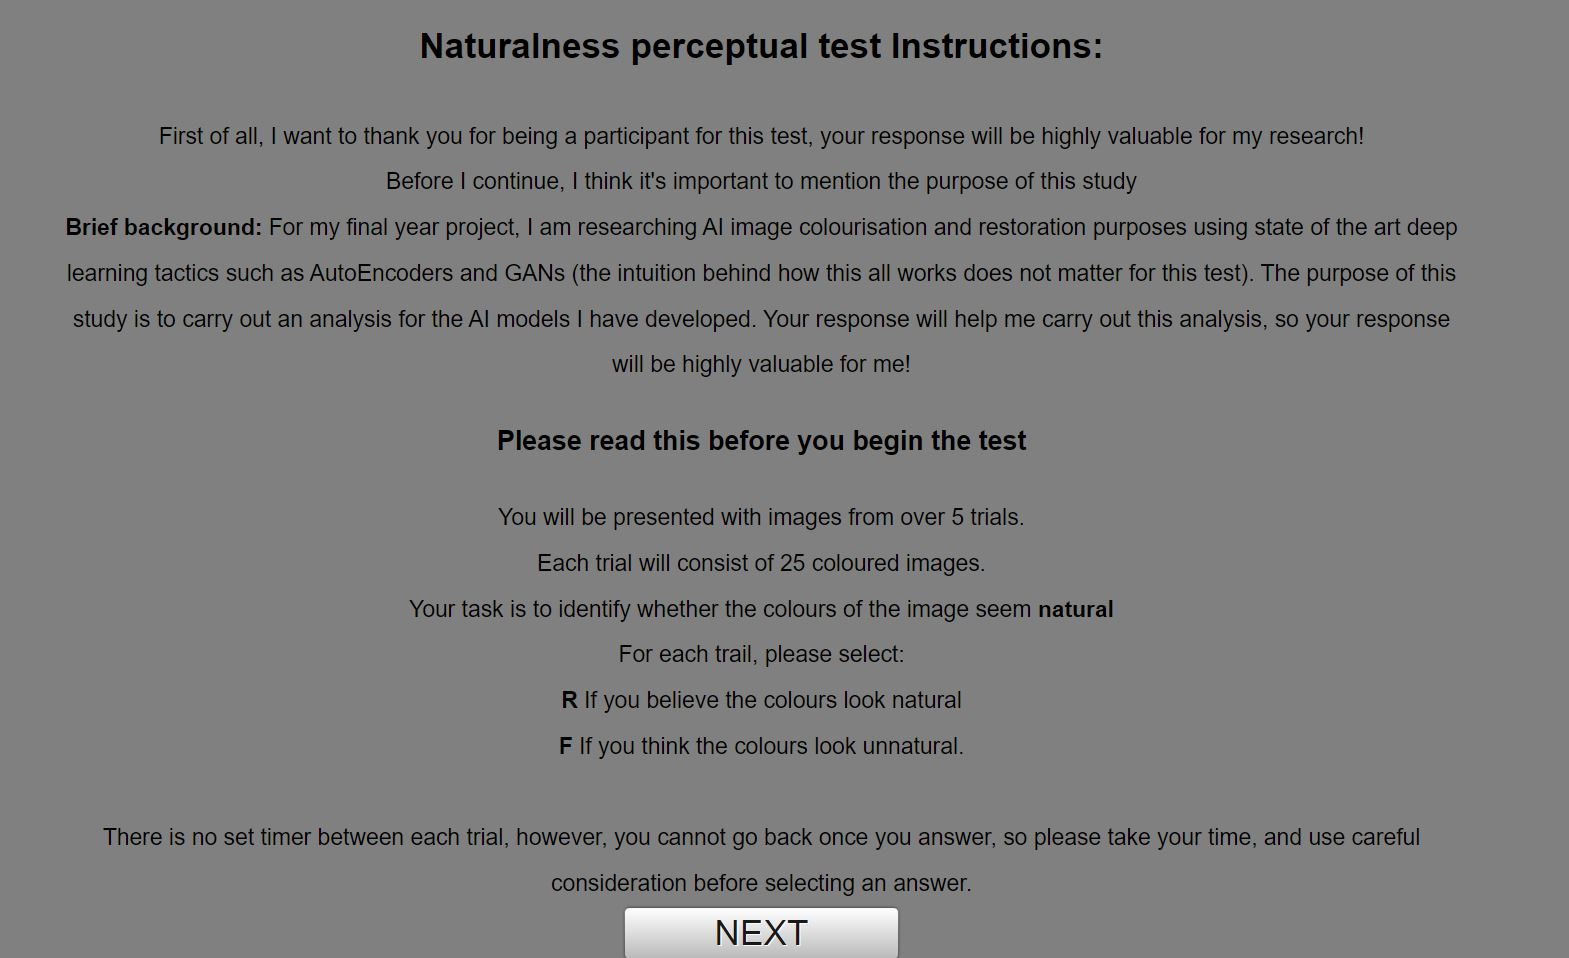
\includegraphics[width=0.8\columnwidth]{sections/figures/naturalness_study_instructions.JPG}
    \caption{Naturalness Perceptual test instructions}
    \label{fig:my_label}
\end{figure}



For example, figure 3.9 is one of the many images presented to the user, they needed to press R or F to answer.

\begin{figure}[H]
     \centering
     \begin{subfigure}[b]{0.3\textwidth}
         \centering
         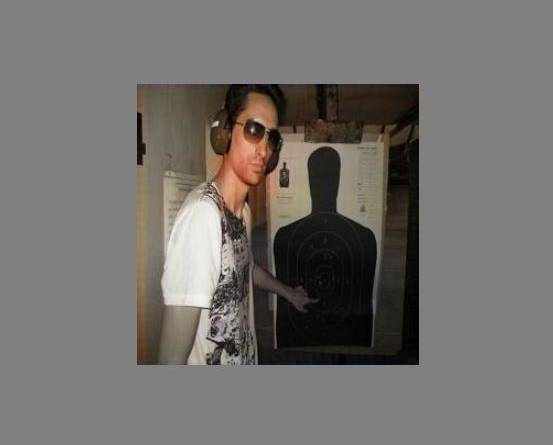
\includegraphics[width=\textwidth]{sections/figures/study_1.JPG}
         \caption{}
         \label{fig:y equals x}
     \end{subfigure}
     \hfill
     \begin{subfigure}[b]{0.3\textwidth}
         \centering
         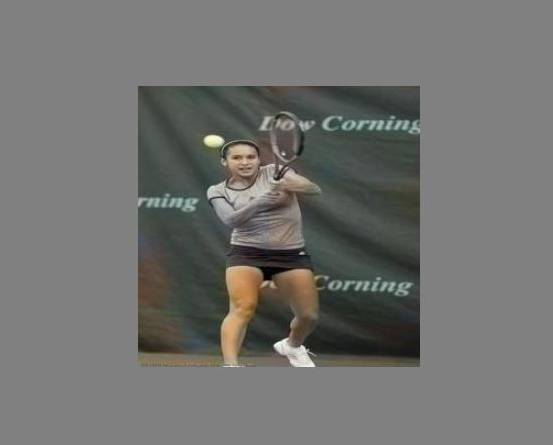
\includegraphics[width=\textwidth]{sections/figures/study_2.JPG}
         \caption{}
         \label{fig:three sin x}
     \end{subfigure}
     \hfill
     \begin{subfigure}[b]{0.3\textwidth}
         \centering
         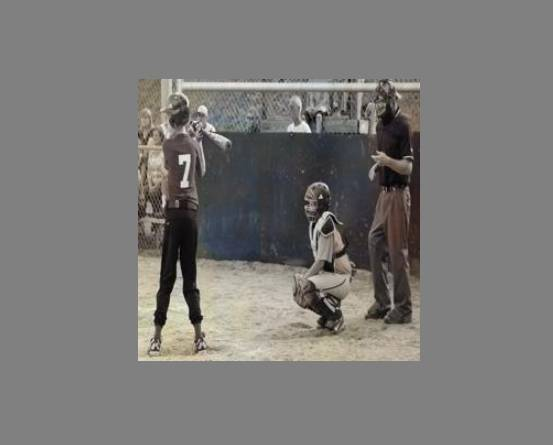
\includegraphics[width=\textwidth]{sections/figures/study_3.JPG}
         \caption{}
         \label{fig:five over x}
     \end{subfigure}
        \caption{Three simple graphs}
        \label{fig:three graphs}
\end{figure}



The study was carried out using a website called \(testable.org\) which is primarily used for experimenting with people's behaviour and perception using surveys and tests. 

This technique was used as calculating accuracy turned out to be unreliable because the calculated accuracy is used to calculate the similarities between two images and does not takes into consideration the naturalness. This could only be achieved by carrying out a study, hence the purpose of this method.











%REFERENCE 1 : https://machinelearningmastery.com/adam-optimization-algorithm-for-deep-learning/#:~:text=Adam%20is%20a%20replacement%20optimization,sparse%20gradients%20on%20noisy%20problems.

%REFERENCE 2: http://kronosapiens.github.io/blog/2017/03/28/objective-functions-in-machine-learning.html

%REFERENCE 3: chrome-extension://cbnaodkpfinfiipjblikofhlhlcickei/src/pdfviewer/web/viewer.html?file=file:///C:/Users/munee/Downloads/electronics-10-00593-v3.pdf

%REFERENCE 4: https://vitalflux.com/hold-out-method-for-training-machine-learning-model/

%REFERENCE 5: https://www.sciencedirect.com/topics/engineering/peak-signal#:~:text=PSNR%20is%20defined%20as%20the,noise%20that%20affects%20representation%20fidelity.

%REFERENCE 6:https://www.matlabclass.com/2014/02/how-to-calculate-psnr-peak-signal-to.html

%REFERENCE 7: https://slurm.schedmd.com/overview.html



    \chapter{Results and Discussion}
This chapter goes over the results gathered for each method. Accuracy, Loss, SSIM, PSNR and Naturalness study are all used to evaluate each method's performance. Each method is also tested and evaluated on the colourisation of historical photos, and restoration of old coloured photos.
\section{Training results}
After training each model for two weeks, their metrics have been recorded. Below are the results gathered from both AutoEncoders and cGAN.




\subsection{AutoEncoder training results}
Both AutoEncoders were trained for 50 epochs. Accuracy and Loss were recorded during training. The \textbf{accuracy} is calculated by totalling up the number of correctly predicted pixels and dividing it by the total number of pixels in the image. The \textbf{Loss} is another way of measuring similarity, and the goal is to minimise this loss.
Both, training and \textbf{validation loss and accuracy} metrics are shown together. The recorded validation metric is used to determine the model's performance.

\begin{center}
\begin{tabular}{||c c c c||} 
 \hline
  AutoEncoder & Val accuracy & Val loss & Optimal epoch \\ [0.5ex] 
 \hline\hline
 Simple AutoEncoder & 67\% &  0.0095 & 50\\ 
 \hline
 Global AutoEncoder & 69\% & 0.00917 & 45\\
 \hline

\end{tabular}
\end{center}

Table 1. Above shows the training results gathered from two AutoEncoder methods. Out of both models, The Global AutoEncoder has performed the best in terms of accuracy (near 70\%) and low loss (0.0091). This suggests that having a global feature extractor can lead to improvements in colourisation.


\subsubsection*{Simple AutoEncoder Loss/Accuracy graph}
\addcontentsline{toc}{subsubsection}{Simple AutoEncoder Loss/Accuracy graph}
\begin{figure}[H]
    \centering
    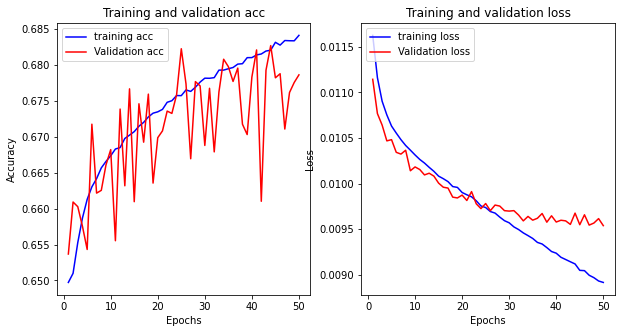
\includegraphics[width=0.7\columnwidth]{sections/figures/autoencoder1_history_loss.png}
    \caption{Simple AutoEncoder training history over 50 epochs}
    \label{fig:my_label}
\end{figure}

In Figure 4.1, you can see the training progress of the Simple Autoencoder. The model was trained for 50 epochs, which took 24 hours to complete. The left graph demonstrates the \textbf{accuracy} for both validation and training sets, while the right graph displays the \textbf{loss} values for both sets. Notice how the validation accuracy has a decent ascending trend, although there is some fluctuation. This is likely due to having a small batch size of 32. The best validation accuracy was \textbf{67\%, achieved at epoch 50}. Whereas the validation loss decreases between 0 and 20 epochs, then levels off and eventually reaches a good \textbf{validation loss of 0.0095} at epoch 50.

\subsubsection*{Global AutoEncoder Loss/Accuracy graph}
\addcontentsline{toc}{subsubsection}{Global AutoEncoder Loss/Accuracy graph}
\begin{figure}[H]
    \centering
    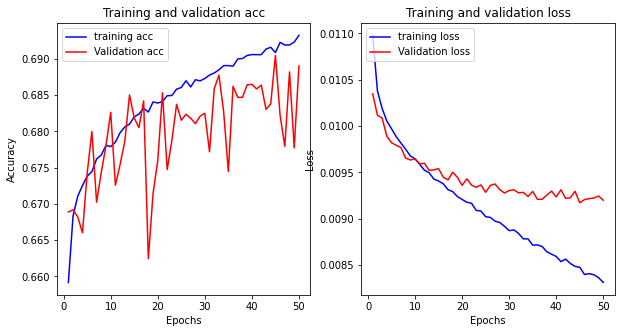
\includegraphics[width=0.7\columnwidth]{sections/figures/autoencoder2_history_loss.png}
    \caption{Global AutoEncoder training history for 50 epochs}
    \label{fig:my_label}
\end{figure}
Here, in Figure 4.2, you can see the recorded history of the Global AutoEncoder training progress. The model has been trained for 50 epochs. However, this method took more time to complete training (2 days) due to it having more parameters to tune. The left graph depicts an upward trend in validation accuracy, though fluctuations continue to be an issue. Whereas in the right graph you can see a similar pattern to the last AutoEncoder, but it drops more quickly and levels out at an early epoch of 10. The \textbf{best validation accuracy was 69\% and loss was 0.0091, which was achieved in epoch 45}.
\subsection{cGan training results}


\begin{center}
\begin{tabular}{||c c c||} 
 \hline
  cGan & Discriminator loss & Generator loss \\ [0.5ex] 
 \hline\hline
 Pix2Pix & 0.0001 & 16.880\\ 
 \hline
 ChromaGAN & -0.0013 & 0.0002\\
 \hline

\end{tabular}
\end{center}
Table 2. The above shows the results gathered for both cGAN methods (Pix2Pix and ChromaGAN). Unfortunately, it is difficult to compare both cGAN models since both rely on entirely different loss metrics as Pix2Pix uses \(L1\) loss whereas ChromaGAN relies on Wasserstein loss for both their generator and discriminator. 

\subsubsection*{Pix2Pix Loss graph}
\addcontentsline{toc}{subsubsection}{Pix2Pix Loss graph}
\begin{figure}[H]
    \centering
    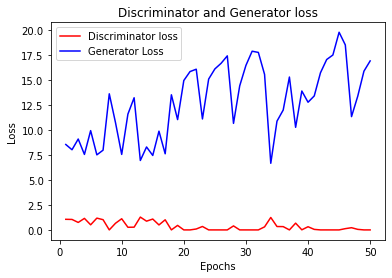
\includegraphics[width=0.7\columnwidth]{sections/figures/pix2pix_history.png}
    \caption{Pix2Pix training history over 50 epochs}
    \label{fig:my_label}
\end{figure}
In figure 4.3, the recorded history of the Pix2Pix cGAN training is shown. The cGAN was trained for 50 epochs, which took 4 days to train using Slurm facility. As observed from the graph, generator and discriminator loss have been plotted. It appears as though the generator is failing to achieve its objective against the discriminator. Despite the generator's loss having an increasing trend, at some points, it has achieved a lower loss, for example in epoch 34. If the model were to be trained for more epochs, the generator would eventually start to win against the discriminator. However, this would take more time for training. Fortunately, I have also trained this model on a smaller dataset (7,000 images) over 400 epochs (refer to Appendix B).

\begin{figure}[H]
    \centering
    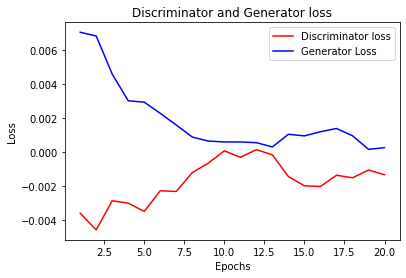
\includegraphics[width=0.7\columnwidth]{sections/figures/chromagan_history.png}
    \caption{ChromaGAN training history for 50 epochs}
    \label{fig:my_label}
\end{figure}
\subsubsection*{ChromaGAN Loss graph}
\addcontentsline{toc}{subsubsection}{ChromaGAN Loss graph}
Figure 4.4 shows the training history for ChromaGAN cGAN. Unlike previous methods, ChromaGAN was only trained for 20 epochs, due to the long training time of 5 days. The generator loss shows a descending trend between the first 8 epochs, then begins to plateau until it ascends slightly between epochs 15 and 17, and then begins to dip again. The discriminator loss mirrors the generator loss. Compared with Pix2Pix, ChromaGAN shows good progress and does not inherit any of the issues seen in the Pix2Pix training history graph, such as the increasing, fluctuating generator loss.








\section{Image colourisation showcase}
\begin{figure}[H]
    \centering
    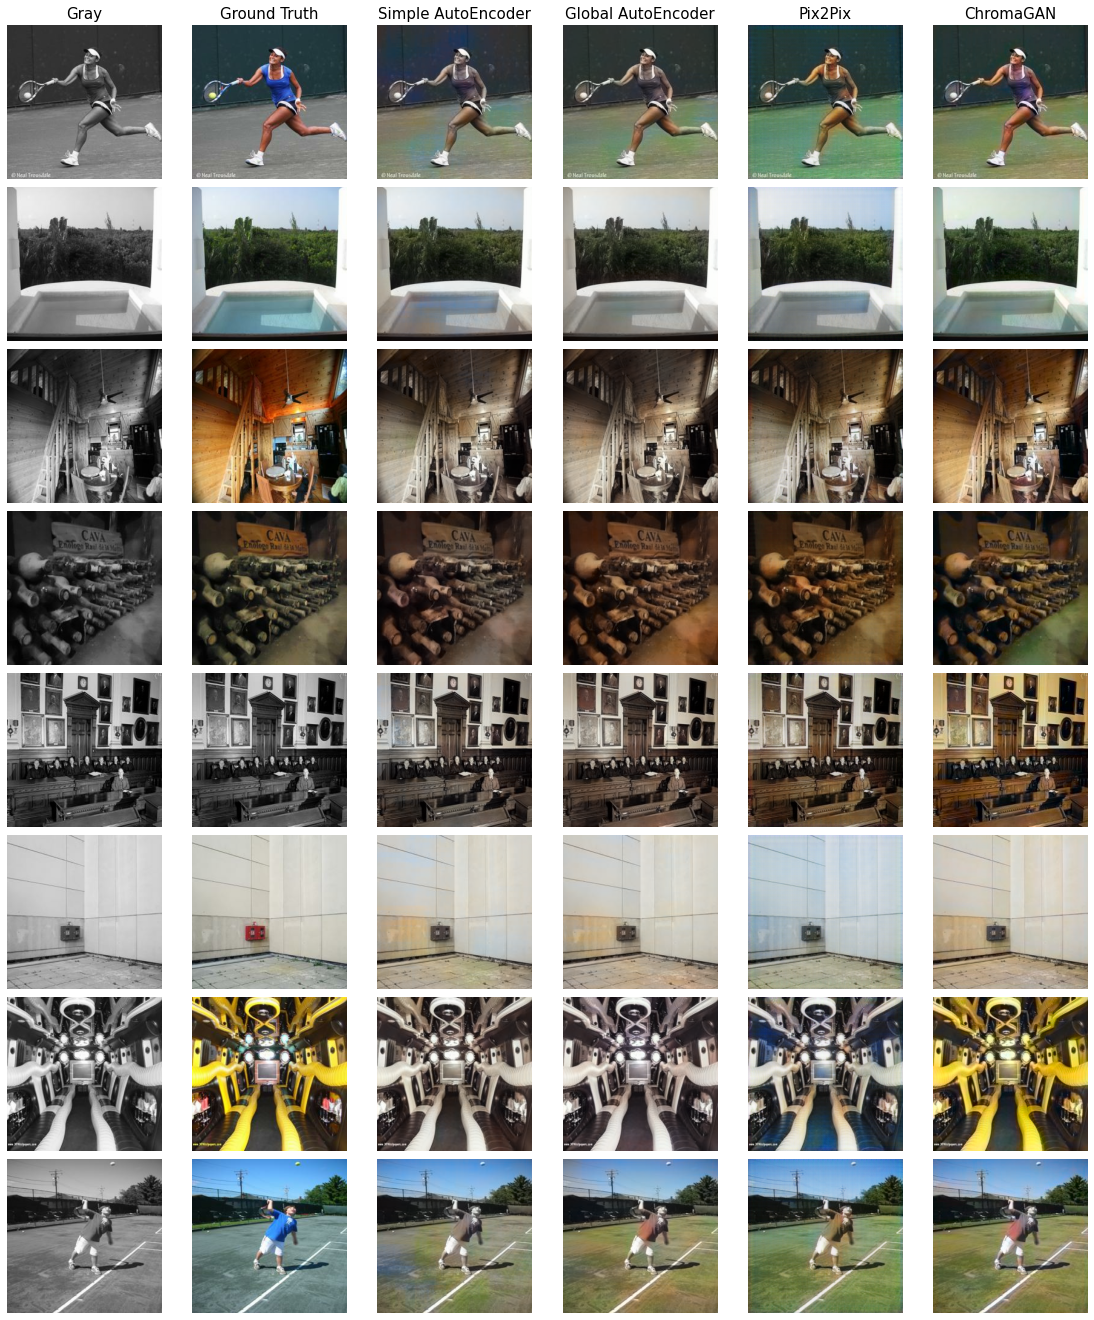
\includegraphics[width=1\columnwidth]{sections/figures/colourisation.png}
    \caption{Eight random images from the test set are colourised. Each row represents an image. The left most column is the grayscale whereas the one next to it is the ground truth. The following three other columns are the three methods used for colourisation.}
    \label{fig:my_label}
\end{figure}


\begin{figure}[H]
    \centering
    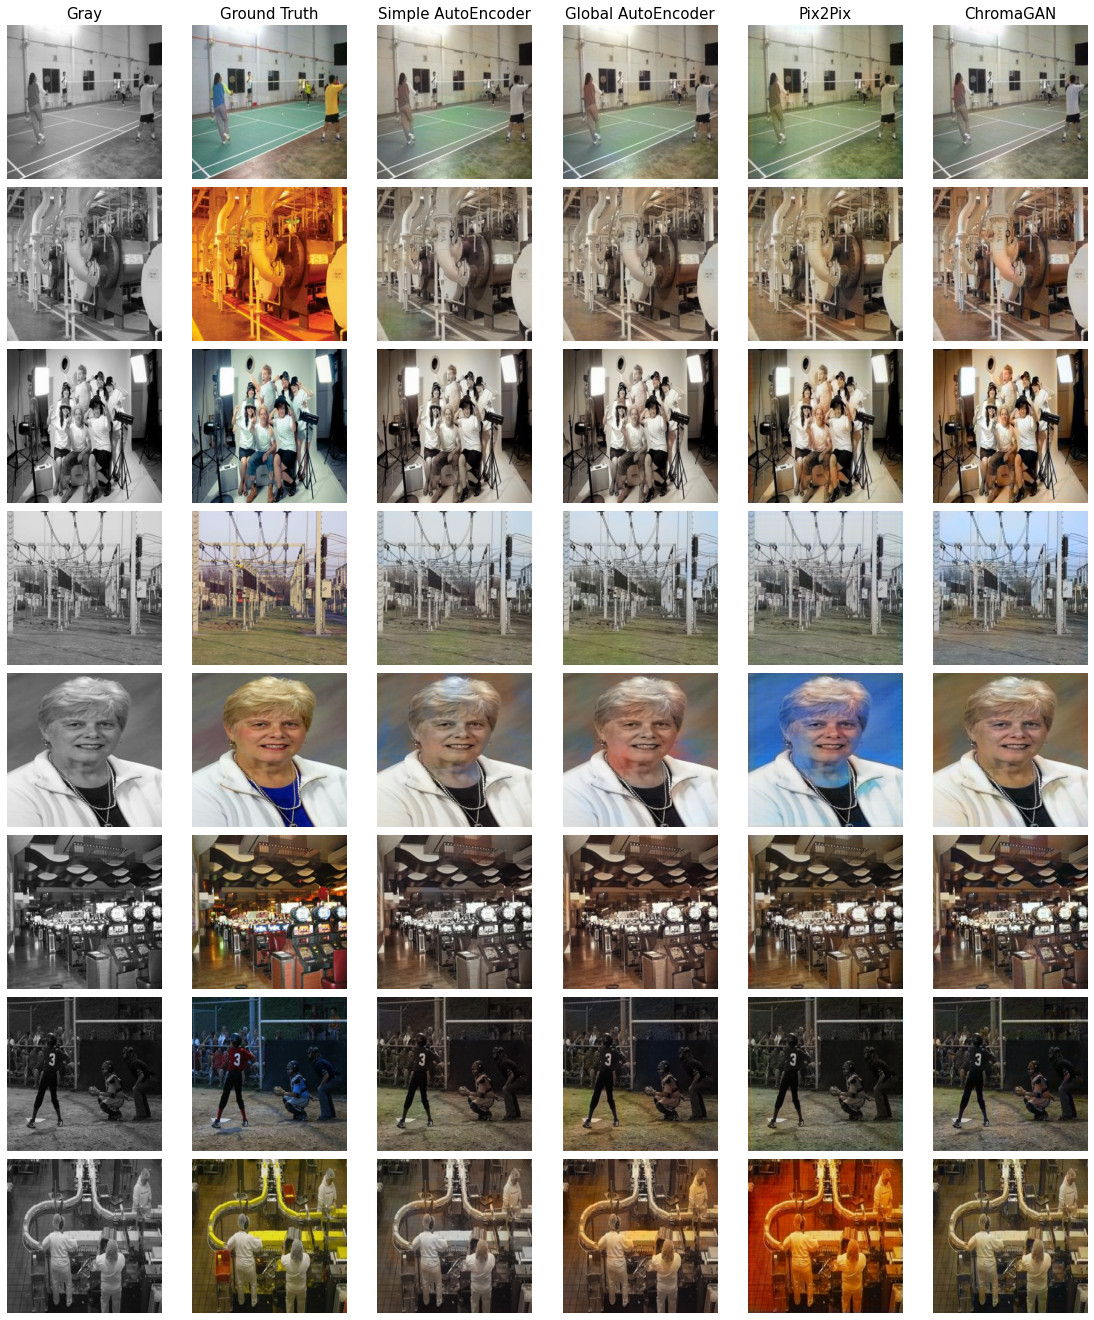
\includegraphics[width=1\columnwidth]{sections/figures/colourisation3.png}
    \caption{Further eight more random images are colourised to showcase each method's colourisation ability.}
    \label{fig:my_label}
\end{figure}



\section{Evaluation}
It was noted in the training results section that accuracy and loss are not reliable metrics to compare between methods since both AutoEncoder and cGAN methods rely on entirely different metrics for evaluation. For this reason, this section will explore evaluation metrics such as \textbf{PSNR}, \textbf{SSIM} and \textbf{natrualness study} which will assist the performance comparison between the methods. 
\subsection{Metric evaluation}
\subsubsection*{Objective score evaluation}
\begin{center}
\begin{tabular}{||c c c||} 
 \hline
  Method & PSNR (dB) & SSIM\\
 \hline
 Simple AutoEncoder & 24.36 & 0.933\\ 
 \hline
 \textbf{Global AutoEncoder} & \textbf{24.45} & \textbf{0.936}\\
 \hline
 Pix2Pix & 23.355 & 0.906\\
 \hline
 ChromaGAN & 23.94 & 0.921\\
 \hline
\end{tabular}
\end{center}
The PSNR and SSIM objective metrics were used to evaluate all mentioned architectures using a test set of 21,000 images.  Here, you can see a correlation between both metrics. For example, the Global AutoEncoder achieves the best PSNR and SSIM score of 24.45 and 0.936 respectively. Whereas, Pix2Pix comes in last, scoring the lowest in PSNR and SSIM scores. Notice how the AutoEncoder class outperforms the cGAN, this may be due to the nature of the AutoEncoder training, which involves iteratively attempts to make the predictions similar and more inclined to the targets, and both, PSNR and SSIM rely on \textbf{similarity}. Whereas the cGAN were trained to make the resulting predictions \textbf{realistic}, which disregards the aim of making it similar, hence why the cGAN performed worse off.


% I evaluated the average PSNR score per method using the test of 21,000 images. PSNR is a metric used to calculate the peak signal-to-noise ratio in decibels between two images. The goal is to maximise the PSNR score. The global AutoEncoder seems to have performed the best and the Simple AutoEncoder closely follows up. ChromaGAN is the third-best model, achieving nearly 24 in average PSNR, whereas Pix2Pix comes last as it scored the lowest. The AutoEncoder class outperforms the cGAN, this may be due to the nature of the AutoEncoder training, which involves iteratively attempts to make the predictions \textbf{similar} and more inclined to the targets, and PSNR score measures the similarity. Whereas the cGAN were trained to make the resulting predictions \textbf{realistic}, which disregards the aim of making it similar, hence why the cGAN performed worse off.


\subsubsection*{Naturalness study evaluation}
\begin{center}
\begin{tabular}{||c c||} 
 \hline
  Method & Naturalness\\
 \hline
 Real Images & 93\%\\ 
 \hline
 Simple AutoEncoder & 45\%\\ 
 \hline
 Global AutoEncoder & 51\%\\
 \hline
 Pix2Pix & 53\%\\
 \hline
 \textbf{ChromaGAN} & \textbf{74}\%\\
 \hline
\end{tabular}
\end{center}
26 participants took part in the naturalness study. The study included real images to provide baseline accuracy. The best performing model was ChromaGAN, which achieved 74\% accuracy. Pix2Pix followed with 53\% accuracy. Global AutoEncoder came in third with 51\%. Simple AutoEncoder had the lowest score of 45\%. None of the methods, however, were able to come close to the real image score of 93\%. This may be due to errors that easily gave away the naturalness of the image. For example, \textbf{visual abstracts} which were seen in the first three methods, also, photos containing humans were turned into zombies as parts of their body remained grey. This was seen throughout the first three models. ChromaGAN managed to perform reasonably well, but the reason it isn't on the same level as real images is likely due to the bland colour palette, which is seen throughout all methods. In contrast to the objective scores, cGAN outperformed the AutoEncoders in this study. This was discussed earlier that the cGAN mainly aims to perform \textbf{realistic} colourisation, which is what this study relies on.



\begin{figure}[H]
    \centering
    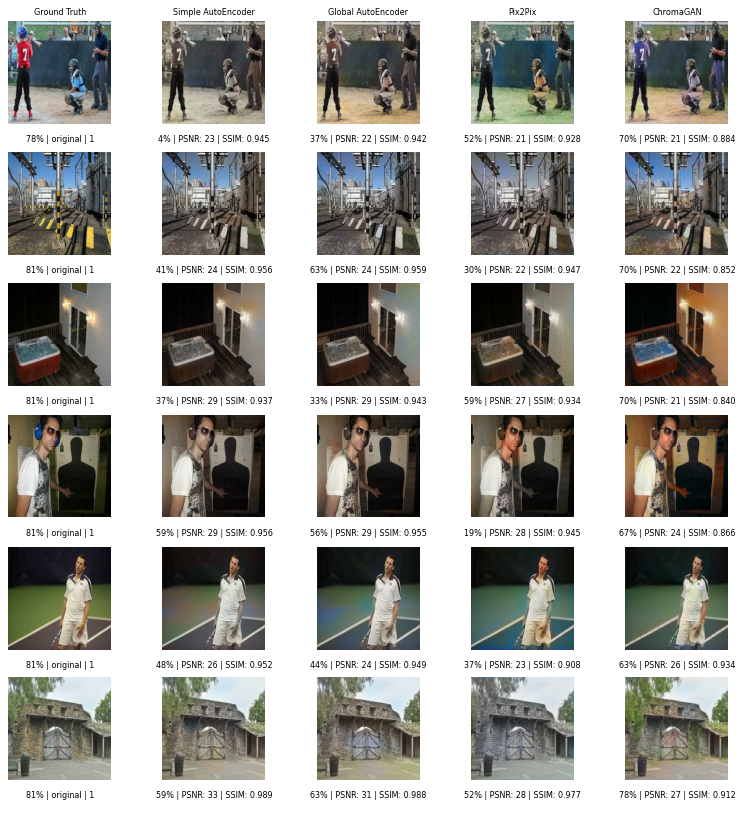
\includegraphics[width=1\columnwidth]{sections/figures/coloured_results.png}
    \caption{For each recoloured image per method, I have added a percentage of users who answered "real" or "fake".}
    \label{fig:my_label}
\end{figure}
Here in Figure 4.5, I've randomly handpicked several images used throughout the naturalness perception study. The left-most column represents the \textbf{ground truth} where the following right columns represent the four methods I have discussed so far. Here, the naturalness percentage score alongside their respective PSNR & SSIM scores.

The first thing I noticed was how the results help depict the behaviour of the observers. For example, some images contain visual abstracts which makes it obvious for the observers to make this "unnatural". Also, some results seem to show little change in percentage even though the contrast or luminosity is slightly tweaked. This shows that the observers are tolerant of minor changes. 

Additionally, you can notice how the cGAN models (pix2pix \& chromaGAN) have performed on average the best in terms of naturalness scores, whereas the two AutoEncoders have scored better in terms of PSNR & SSIM. As discussed in the last section, there does seem to be a clear trade-off between the objective metrics and Naturalness scores. It's fair to assume that the cGAN is likely to be the preferred method even if it has a worse average PSNR & SSIM score. \textbf{In my opinion the scores observed from the human eye (naturalness study) matter more than the scores computed by the computer (PSNR & SSIM)}. Out of all methods, it's observed that the ChromaGAN is the best-suited model for image colourisation. 





\pagebreak
\subsection{Historical photos analysis}
\begin{figure}[H]
    \centering
    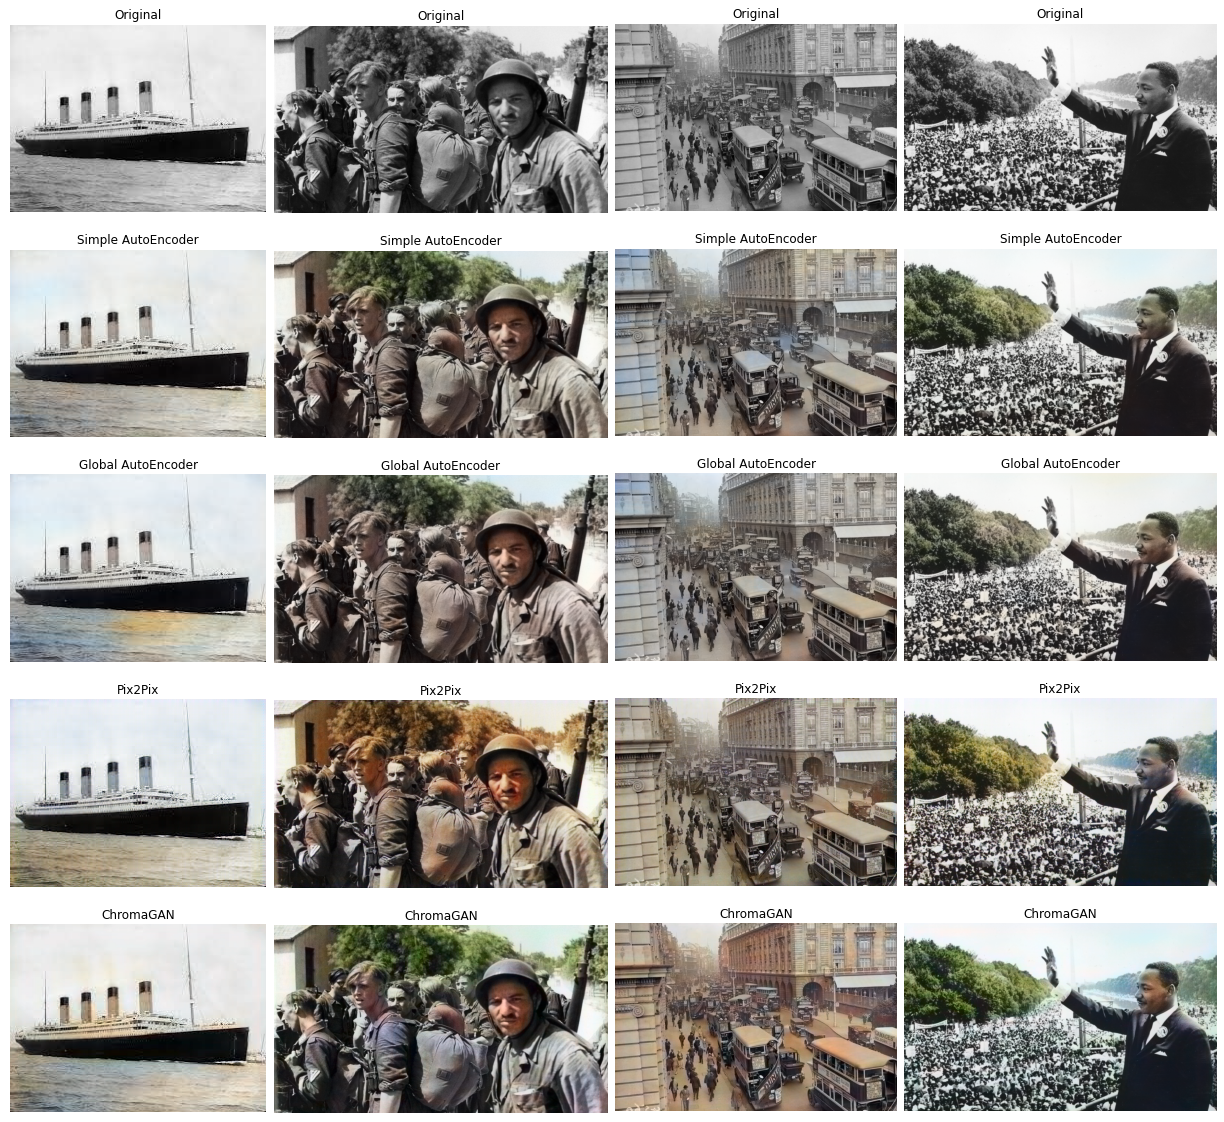
\includegraphics[width=1\columnwidth]{sections/figures/historical_colourised_photos.png}
    \caption{A few historical photos have been picked. Titanic (1912),  French Algerian soldier Gaurding captured German soldiers (1944) and London (1920s), Martin Luther King giving a speech (1963).}
    \label{fig:my_label}
\end{figure}
I've tested each model on historical photos. Figure 4.8 shows the colourisation results. Since there are no ground truths to identify how accurate each model is, it is down to personal judgement. ChromaGAN seems to show the best overall colourisation results as it does a better job colourising people and their surroundings. 

\subsection{Colour restoration analysis}

\begin{figure}[H]
    \centering
    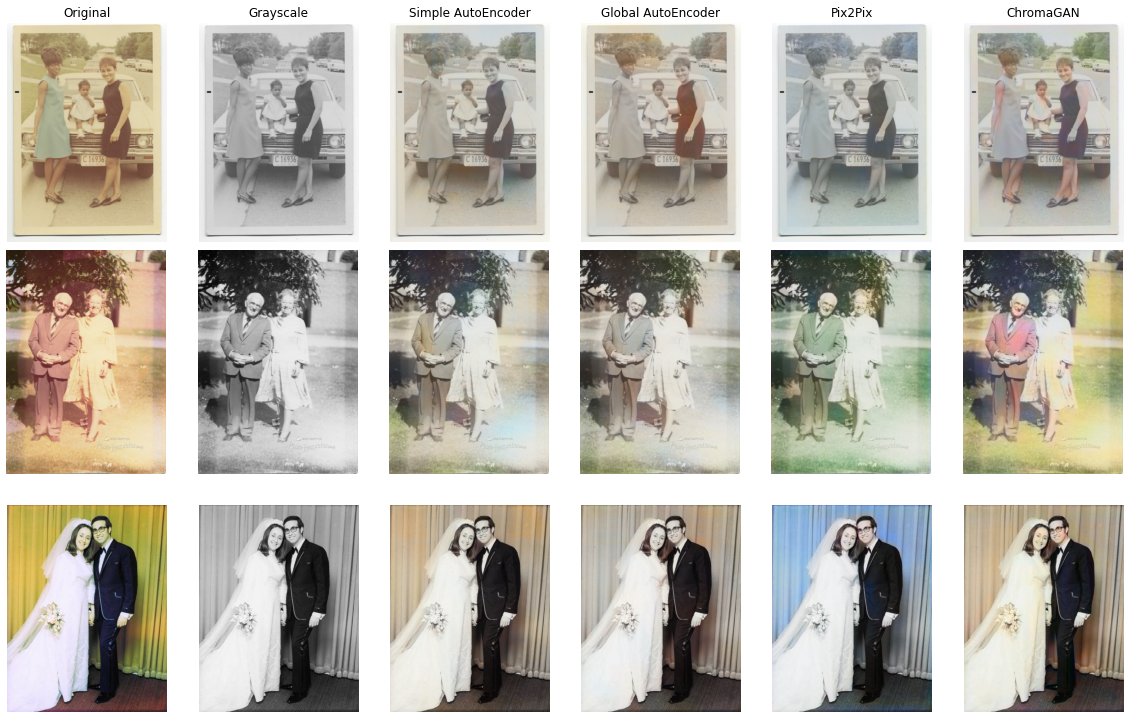
\includegraphics[width=1\columnwidth]{sections/figures/colour_resortation.png}
    \caption{Restoring the colours of a few photos whose colours have faded}
    \label{fig:my_label}
\end{figure}


 I've handpicked three photos that have suffered deterioration in quality due to environmental factors such as poor handling, poor material or ageing. The photos were used to test each model's capabilities for the purpose of restoring colours. 

 Out of all methods, the ChromaGAN model has done a decent job in bringing back the vibrant colours which lacked in the original photos. It even removed the orange hue seen within the first two original images.

 However, not all methods are accurate, for example in the third row, Pix2Pix coloured the curtains blue instead of yellow. 

 It is also important to note that the models cannot remove the fade effect or any other visual abstracts seen in the original image as none of the models were trained to deal with this type of issue, hence why its presence still exists in the resulting images. 
\pagebreak
\section{limitations}
\begin{figure}[H]
    \centering
    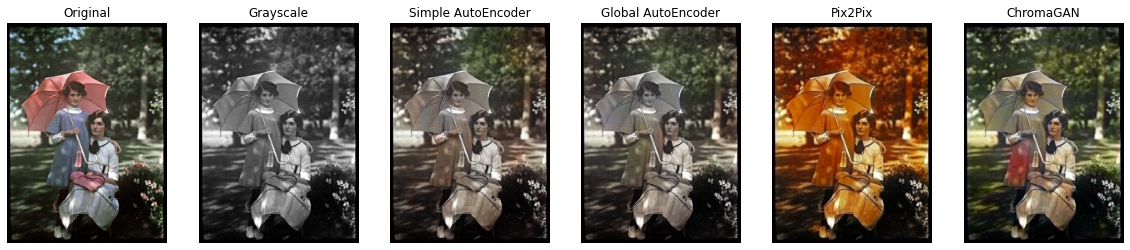
\includegraphics[width=1\columnwidth]{sections/figures/limitation1.png}
    \caption{Limitation example 1}
    \label{fig:my_label}
\end{figure}
Here, it is important to outline a few key limitations observed from all methods. For example, figure 4.10 demonstrates some form of the limitations suffered by each model:

\begin{enumerate}
  \item All methods were trained to colourise images of size 256x256 (except ChromaGAN - 242x242), this means that test images require resizing. Resizing causes distortion which can negatively impact the colourisation process. This is seen in the first three methods.
  \item The colourisation process is biased and will not apply accurate colours to everything. For instance, it failed to colourise the umbrella or the handbag pink. This is because the algorithms were only trained on what they had seen and likely never trained on images consisting of pink umbrellas and pink handbags. 
  \item The predicted colours are also bland, especially complex small objects. This again relates to the last point of bias: The algorithm has a lot to learn before it can learn to colourise more entities using accurate colours.
  \item Incorrect colour placement and visual abstracts are very apparent and seen throughout all models. For instance, the colourisation of Pix2Pix is completely all orange, whereas ChromaGAN has produced a slight reddish visual abstract which can be seen on the dress of the left person. 

\end{enumerate}
Despite mentioning all these limitations, some of the methods such as ChromaGAN manage to do a decent enough job to make the colourisation look convincing, however, still suffer from the limitations mentioned above.




\begin{figure}[H]
    \centering
    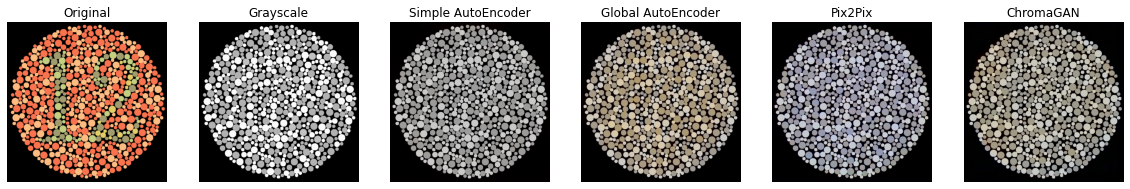
\includegraphics[width=1\columnwidth]{sections/figures/limitation2.png}
    \caption{Limitation example 2}
    \label{fig:my_label}
\end{figure}
Furthermore, the methods are not suitable for colourising synthetic images as demonstrated in figure 4.11. For instance, the colour blind test contains a "12" which is coloured in green. However, as you can observe, the grayscale image completely loses all the information of all the synthetic colours, and if we, the viewers can not see a "12" from a grayscale image then neither can the models. 

\pagebreak
\section{Discussion}
Let's revisit the aims established at the beginning of this investigation:

\begin{enumerate}
  \item Determine the best image colourisation method by carrying out an analysis of deep learning architectures such as AutoEncoders and Conditional Adversarial Networks using quantitative measures such as human assessment and objective metrics.
  \item Investigate whether the objective measures correlate with
human assessment results and determine which measures matter more for the purpose of image colourisation.
\end{enumerate}

Now I believe the first aim has been addressed since judging from the results discussed earlier, I've successfully carried out an analysis of AutoEncoders and cGAN using objective measures (PSNR & SSIM) and human measures (natural perception test). Here, judging from the results, it appears that the cGAN methods provide more realistic results, offering diverse colourisation than AutoEncoders, while AutoEncoders generate results that better match the targets but with colours often seen as less realistic. Here, it was revealed that the human assessment tends to rely more on realistic colourisation, whilst the objective measures relied more on similarity. And it was seen that the cGAN performed better on realism, whereas AutoEncoders were better are similarity.

So there's a clear trade-off between realism and similarity, which raises the second aim established earlier. It's clear that the objective measures do not correlate with human opinion, and this may be because the objective measures only focus on the structural and noise differences, not the colour, which the human volunteers focused on, which makes the objective metrics unreliable in conducting an evaluation for image colourisation. Unfortunately, there does not seem to be any alternative metrics, hence using human-driven study was needed.   

Also, according to this study, ChromaGAN performed consistently the best as it managed to achieve the highest average naturalness study score (73\%) and a reasonably good average PSNR/SSIM score, making ChromaGAN the best-suited algorithm for image colourisation.





    \chapter{Conclusions}
The purpose of the research was to study and analyse different deep learning methods, specifically AutoEncoders and cGANs. The AutoEncoders used were Simple and Global AutoEncoder, both based on the Authors of \cite{deepkoal2017}. Pix2Pix and ChromaGAN were chosen to investigate the performance of cGAN and used to compare against the AutoEncoder methods explored earlier. 

The Places365 dataset was used to train all methods. The dataset consisted of 105,000 samples split into a 60:20:20 ratio. A TensorFlow pipeline was used to help work with the large dataset while having limited memory space. I chose to train the models in Slurm Facility, a service provided by the university that is practically free. 

After a couple of days of training, the methods were tested on the reserved test set and evaluated using objective metrics and Naturalness study. Results have shown that AutoEncoders tend to perform better than cGAN methods using objective metrics, but cGAN performed better on Naturalness Study. 

This raised questions about which evaluation metric matters more. It was noted known that using objective metrics were not reliable when dealing with coloured images as it would only focus on structural and noise difference, not the colour. Hence, the only useful way of evaluating the methods was through human opinion via naturalness study. This study helped conduct a more fair comparison between all methods. The results of the study showed that cGAN was the best deep learning method out of the two compared.




% AutoEncoders are likely biased, as in nearly all cases cGAN manages to perform better in providing more realistic and natural colours. Using historical and colour restoration analysis, and using naturalness study helped reduce this bias and conduct a more fair comparison between all methods. The results of the study showed that cGAN was the best deep learning method out of the two compared.





\section{Future Work}
\subsection{More Data}
One of the limitations seen throughout this project was the time constraint which forced me to limit the dataset to a rather small size of 80,000. And even then, training took a considerable amount of time, taking at most 5 days for training one method (ChromaGAN) for only 20 epochs. Even though \textbf{80,000} may sound a lot in other deep learning tasks, it isn't sufficient enough for the task of Image Colourisation. Having more data will enable the model to achieve a far richer hyperspace to leverage from, which may achieve far more impressive colourisation results.

\subsection{NoGAN training}

\begin{figure}[H]
    \centering
    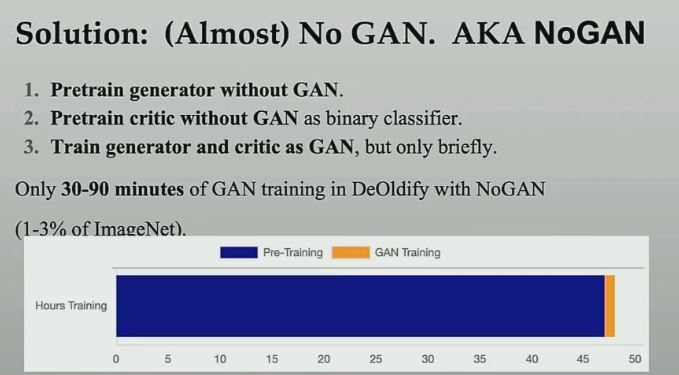
\includegraphics[width=0.8\columnwidth]{sections/figures/nogan.JPG}
    \caption{NoGan training process \cite{nogan2020}}
    \label{fig:my_label}
\end{figure}

NoGAN training is another technique used by the authors of Deoldify \cite{nogan2020}. The process is rather straightforward, you first train the generator model by itself and then generate images from that. You then proceed to use those generated images alongside real images and train the discriminator in a binary classification manner. Finally, you briefly train both the generator and the discriminator together in a GAN setting. The effects of this training method are noted to have reduced the visual abstracts seen prior to this method and have overall improved the colourisation quality. 

\subsection{User guided and Exemplar methods}
\begin{figure}[H]
    \centering
    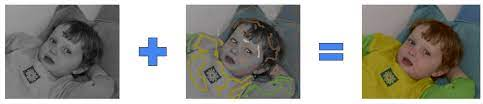
\includegraphics[width=1\columnwidth]{sections/figures/scribble_based_colourisation.jpg}
    \caption{Scribble-based colourisation method which relays on user input \cite{deepimagecolorizationwithuserguidence}}
    \label{fig:my_label}
\end{figure}
Lastly, I would like to experiment with models that involve user guidance. For example, the author's of Scribbler rely on user guidance. The basic process involves scribbling (hence the name) colours onto a chromatic photo. The algorithm will then distribute the colours across regions of the photo. These regions can be anything, such as T-shirts, furniture or landscapes. 

\begin{figure}[H]
    \centering
    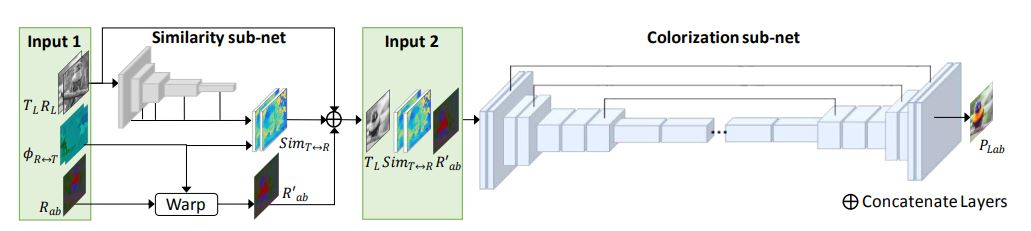
\includegraphics[width=1\columnwidth]{sections/figures/deep_exempler_based_architecture.JPG}
    \caption{Exempler-based architecture for image colourisation \cite{DBLP:journals/corr/abs-1807-06587}}
    \label{fig:my_label}
\end{figure}

In addition to this, I would like to explore ensemble methods that involve combining many models to seek better predictive performance. For example, the author of Deep Exemplar-based Colorization use this technique \cite{DBLP:journals/corr/abs-1807-06587}. 

\section{Self Evaluation}
This research project has allowed me to improve my skills and deepen my interest in the topic of deep learning within the field of Artificial Intelligence. Before beginning this research, I had very little knowledge of AI image colorization or AI in general. The AI and Machine learning modules I took for my third year provided me with the basic foundations I needed to pursue this project. Of course, there were some difficulties along the way: I lacked some key concepts that made understanding certain aspects difficult. However, this was solved after I learnt some of the essential terminologies and concepts. Overall, this project has been an amazing opportunity to learn many new skills and knowledge.


    %TC:ignore 
    \chapter*{A Appendix}
\addcontentsline{toc}{chapter}{A Appendix}  
\section*{Code repository}
If you wish to reproduce the results produced from this investigation, I have a GitHub repository which can be found at the following link:

https://github.com/mrehmm001/Deep-Image-Colourisation-comparing-AutoEncoders-and-Conditional-Adversarial-Networks

A dedicated Nvidia GPU is required to enabled GPU accelaration in order to reduce training time. Also, the dataset I've used was from the places365 website which can be found at the followng URL:

http://places2.csail.mit.edu/download.html

Here, I've used "Places-Extra69" version which contains fewer images of 105,000 total. I've partitioned my owned dataset, and if you wish to use mine, here is the URL link:

https://drive.google.com/file/d/178mTebcMLPT5CixUzJOzoDYDLFpVIyNb/view?usp=sharing

I've used author's code to help conduct this research \cite{deepkoal2017code}, \cite{vitoria2020chromagancode}, \cite{vitoria2020chromagancode}.
\pagebreak


\section*{My research}
\begin{figure}[H]
    \centering
    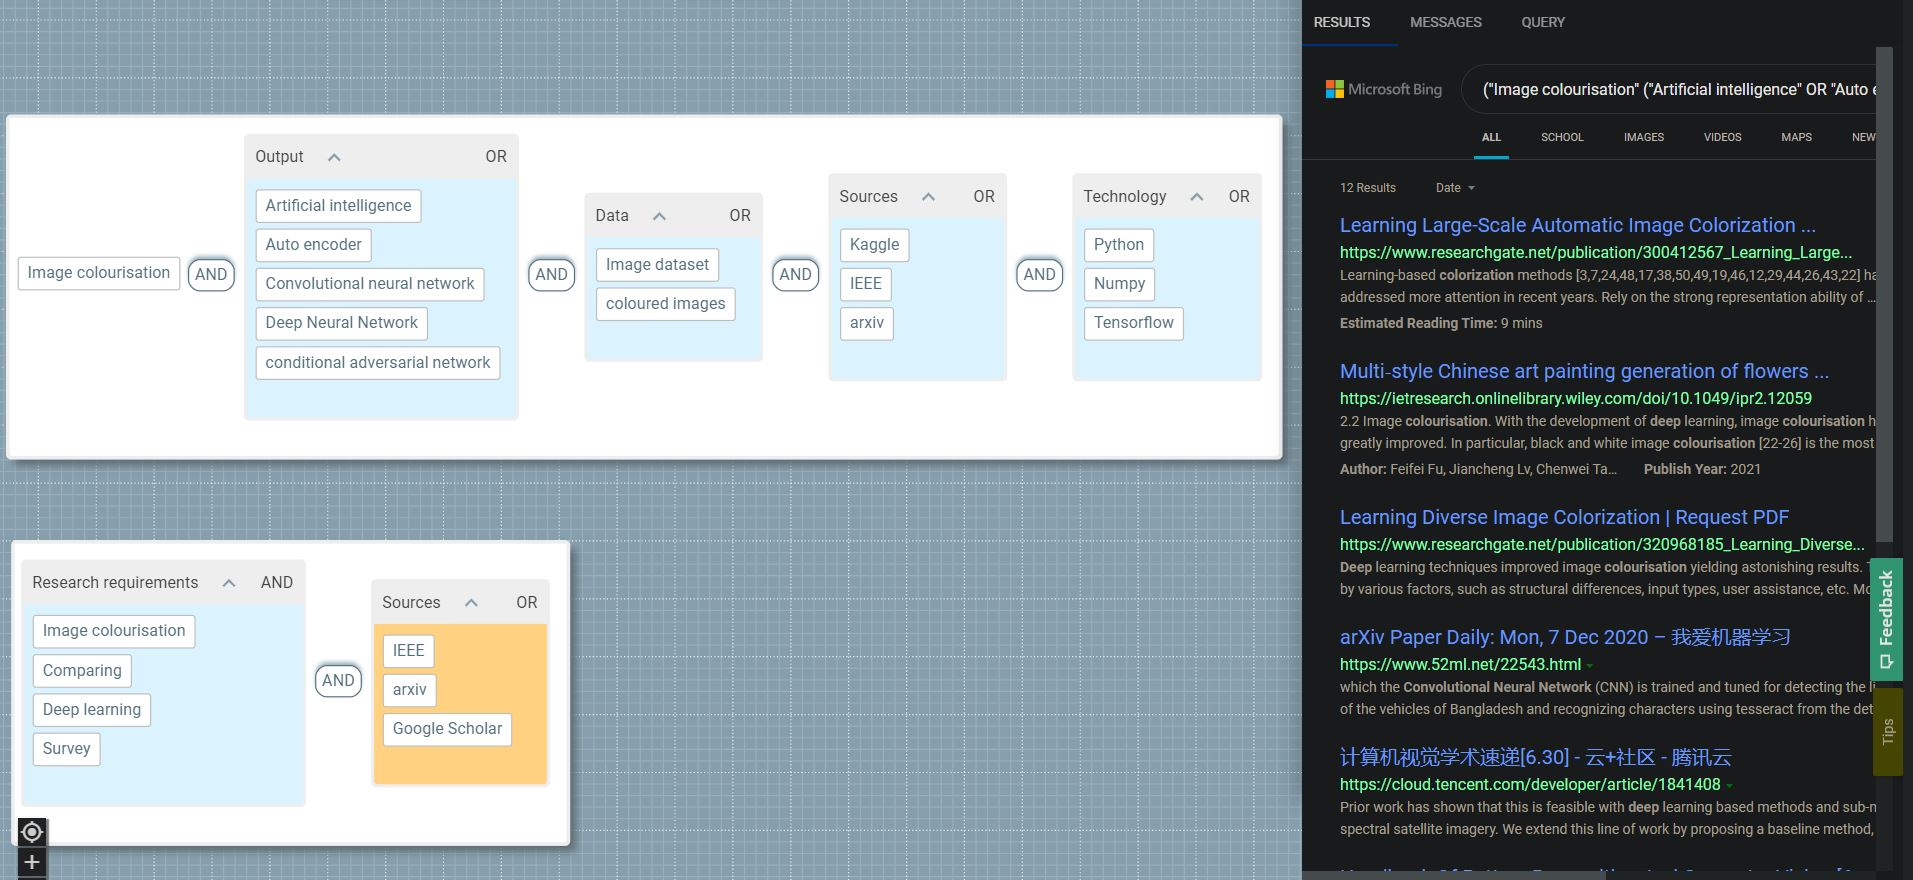
\includegraphics[width=1\columnwidth]{sections/appendix/my_research.JPG}
    \caption{2dsearch was used to help conduct my research}
    \label{fig:my_label}
\end{figure}

\begin{figure}[H]
    \centering
    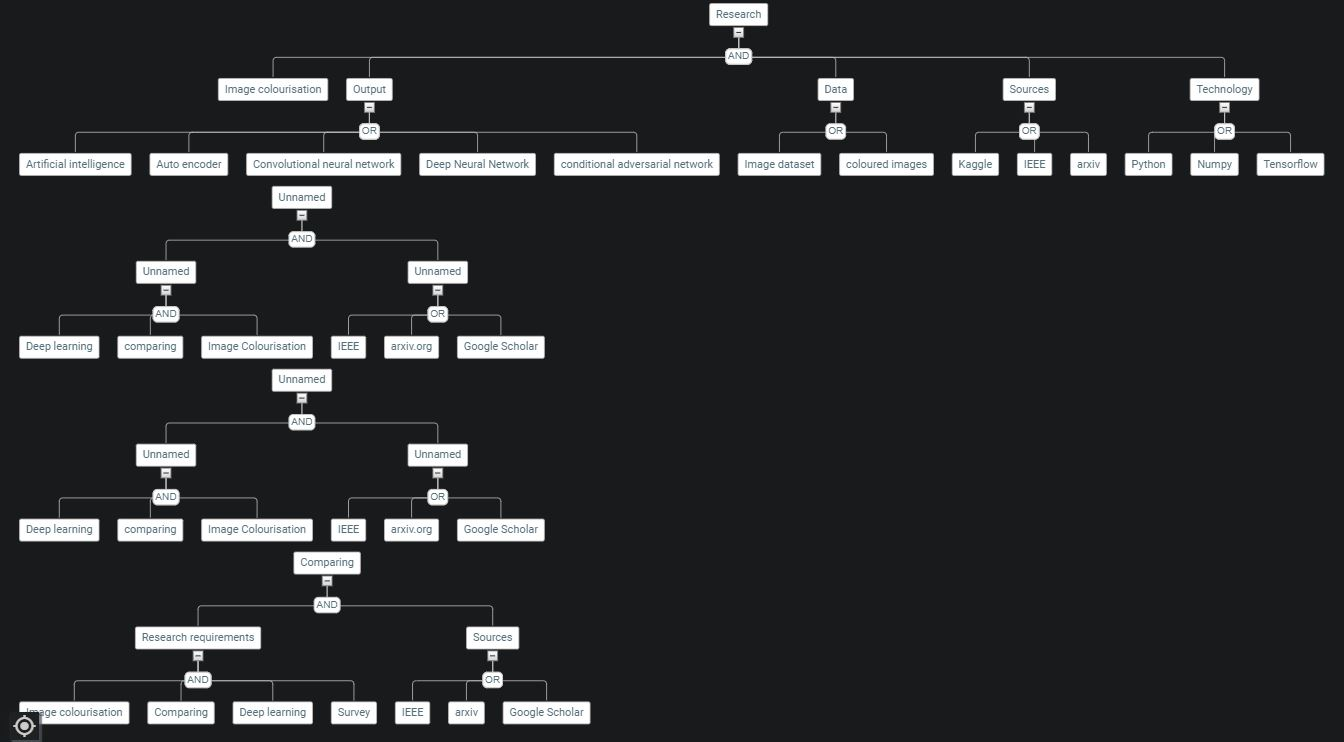
\includegraphics[width=1\columnwidth]{sections/appendix/my_research_tree.JPG}
    \caption{Literature Research tree diagram}
    \label{fig:my_label}
\end{figure}
\newpage
\chapter*{B Appendix}
\addcontentsline{toc}{chapter}{B Appendix}  

\section*{Neural Networks} 
% \lipsum[1-2]
The Artificial Neural Network (ANN) is a structure that is inspired by the human biological brain, it consists of several processing units (neurons) that have a natural propensity for storing experiential knowledge and making it available for use. As S. Haykin puts it, an ANN resembles the human brain in two respect \cite{haykin2009neural}:
\begin{enumerate}
  \item Knowledge is acquired by the network from its endowment through a learning process. 
  \item interneuron connection strengths, known as synaptic weights, are used to store the acquired knowledge.
\end{enumerate}



\begin{figure}[H]
    \centering
    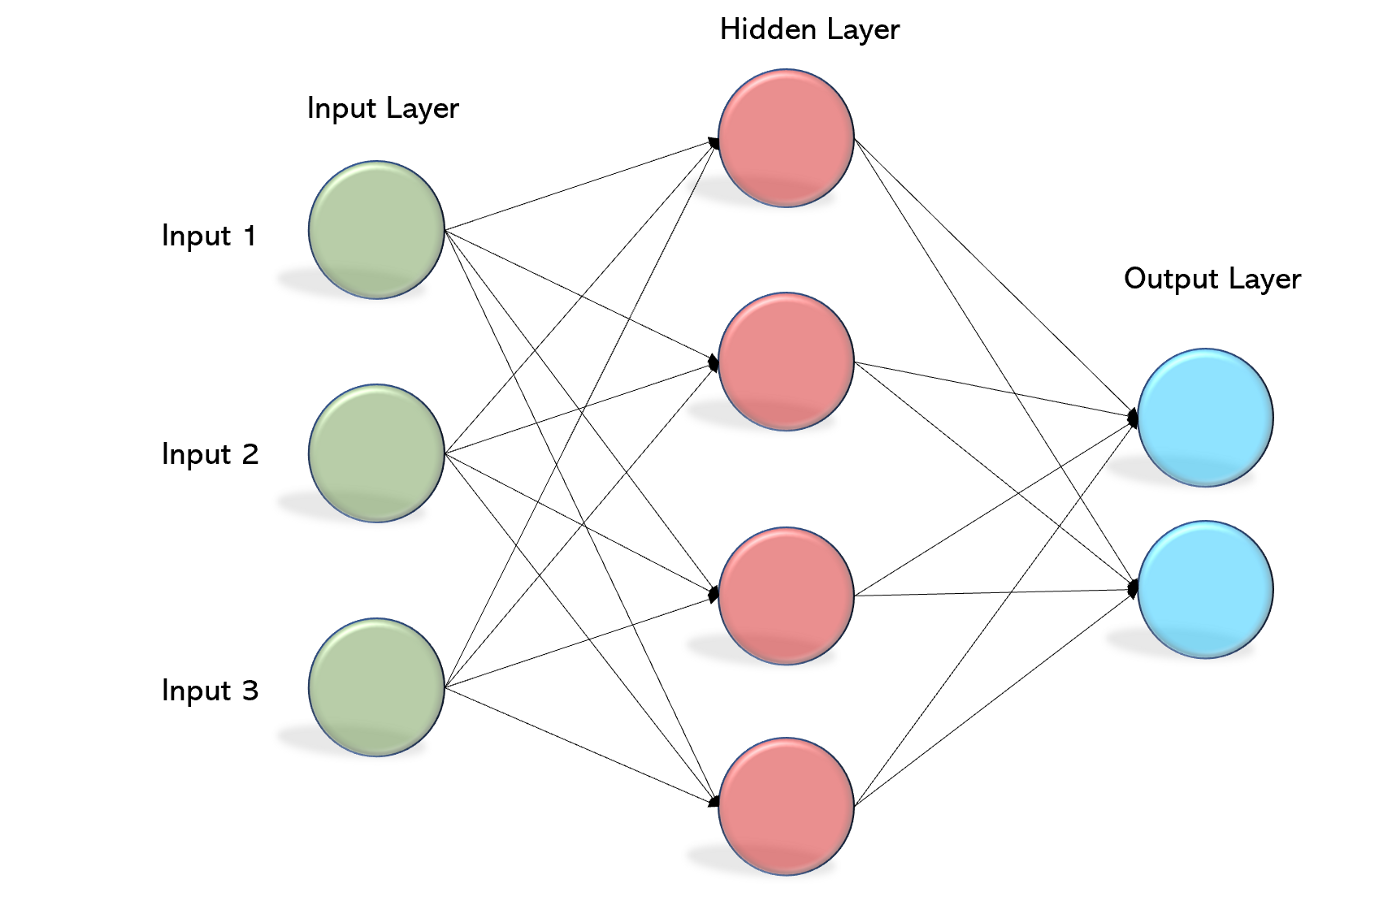
\includegraphics[width=0.5\columnwidth]{sections/figures/mlp.png}
    \caption{Example of a Artificial Neural Network \cite{mohanty_2019}}
    \label{fig:my_label}
\end{figure}

The learning operation that is used to carry out the action is known as the learning algorithm. The learning algorithm is used during the training phase to modify the synaptic weights of the network. The modification of the synaptic weights will influence the behaviour of the network, which will determine the output of the network.



During the training phase, we have training sets that contain input data with corresponding targets. The input data is fed into the network, and the network performs a process called feedforward. Feedforward involves the summation of synaptic weights and corresponding inputs with the application of activation functions. This results in a predicted output. The predicted output is compared against the actual target output and an error is calculated. This error is used to determine how accurate the network was. If the predicted output is wrong, the network uses a learning algorithm known as the backpropagation algorithm. The backpropagation algorithm computes the gradient descent by calculating the derivative and updating the synaptic weights. This process repeats until the learning algorithm converges into what is known as a global minimum. At the global minimum, learning will cease to proceed. This means the network can classify any input and map it to their corresponding predictions that match the targets.




\subsection*{Convolutional Neural Networks}
% \lipsum[1-2]
Convolutional Neural Network (CNN) (also known as convnets) are a special class of ANN used in deep learning and are universally used for computer vision purposes \cite{enwiki:1085146109}. CNN is similar to dense neural networks in ways that CNN consists of input and output layers, as well as several hidden layers, however, the difference lies in the layer: The layer of the CNN consists of a special type of layer called "convolutional layer" (hence the name CNN derives from) that are used to filter out features from the previous layer, called a feature map. The layers also consists of pooling layers which function to reduce the spacial representation size to reduce the number of parameters of the network. The effects of these layers enable CNN to extract complex features from data and learn the representations using fewer parameters, making CNN more efficient at the task of computer vision compared to traditional dense ANN. 

\begin{figure}[H]
    \centering
    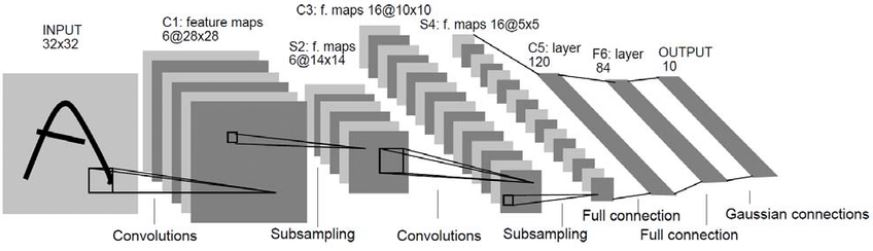
\includegraphics[width=0.7\columnwidth]{sections/figures/cnn.JPG}
    \caption{handwriting recognition using CNN \cite{berus_2018}}
    \label{fig:my_label}
\end{figure}



For further information on how Neural Networks word, refer to Haykin's Neural Network textbook \cite{haykin2009neural} amd deep learning with python \cite{franoischollet2017learning}.


\pagebreak
\section*{Tuning results}
The table shown below demonstrates the AutoEncoder tuning results but on a much smaller dataset (Landscapes by blackmamba \cite{landscape}) which contains in total 8,000 images split 60:20:20 ratio. The results are taken from my interim report \cite{mrehm001}. 
\begin{table}[H]
\Huge
\bfseries
\def\arraystretch{2}
\setlength{\tabcolsep}{10pt}
\begin{adjustbox}{width=\textwidth}
\begin{tabular}{|l|l|l|l|l|l|l|}
\hline
Experiments & Optimal epoch & Val loss & Val accuracy & Batch norm & Augmentation & Learning rate \\ \hline
Experiment 1 & 27 & 0.0096 & 0.6548 & No  & No  & Default (1e-3) \\ \hline
Experiment 2 & 14 & 0.0075 & 0.7155 & No  & No  & 1e-4           \\ \hline
Experiment 3 & 21 & 0.0075 & 0.7065 & No  & No  & 1e-5           \\ \hline
Experiment 4 & 85 & 0.0073 & 0.7106 & Yes & Yes & 1e-4           \\ \hline
Experiment 5 & 62 & 0.0071 & 0.7177 & No  & Yes & 1e-4           \\ \hline
\end{tabular}

\end{adjustbox}
\caption{Experiments gathered throughout the training of the model}
\end{table}

\begin{figure}[H]
    \centering
    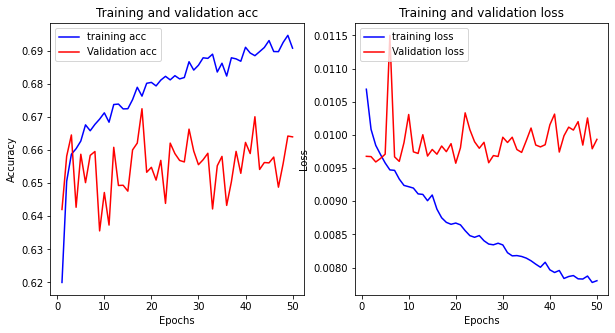
\includegraphics[width=0.7\columnwidth]{sections/figures/Experiment1.png}
    \caption{Experiment 1 plot}
    \label{fig:my_label}
\end{figure}

\begin{figure}[H]
    \centering
    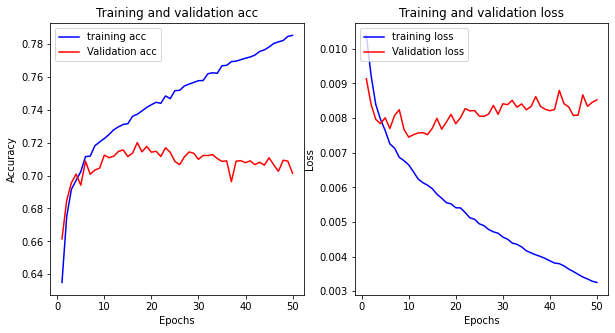
\includegraphics[width=0.7\columnwidth]{sections/figures/Experiment2.png}
    \caption{Experiment 2 plot}
    \label{fig:my_label}
\end{figure}

\begin{figure}[H]
    \centering
    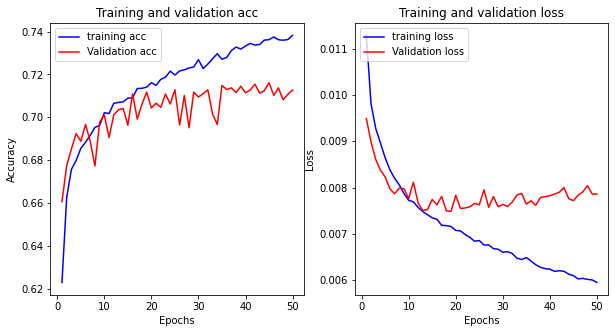
\includegraphics[width=0.7\columnwidth]{sections/figures/Experiment3.png}
    \caption{Experiment 3 plot}
    \label{fig:my_label}
\end{figure}

\begin{figure}[H]
    \centering
    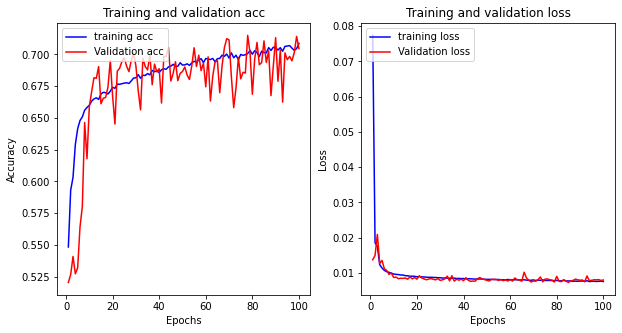
\includegraphics[width=0.7\columnwidth]{sections/figures/Experiment4.png}
    \caption{Experiment 4 plot}
    \label{fig:my_label}
\end{figure}

\begin{figure}[H]
    \centering
    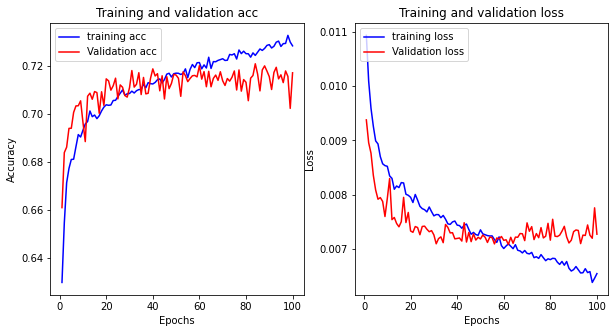
\includegraphics[width=0.7\columnwidth]{sections/figures/Experiment5.png}
    \caption{Experiment 5 plot}
    \label{fig:my_label}
\end{figure}

\subsection*{Optimal model analysis}
\begin{figure}[H]
    \centering
    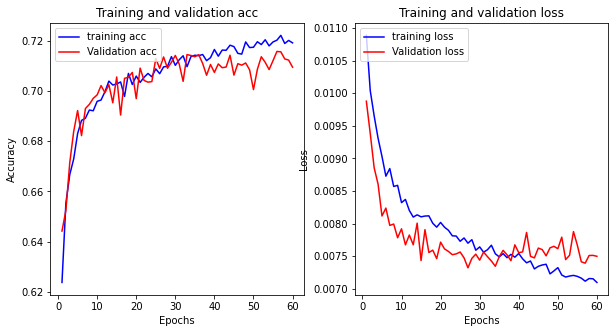
\includegraphics[width=1\columnwidth]{sections/figures/optimal.png}
    \caption{Validation and accuracy plots of the optimal model}
    \label{fig:my_label}
\end{figure}

\section*{Training the Pix2Pix using a smaller dataset}
\begin{figure}[H]
    \centering
    \includegraphics[width=1\columnwidth]{sections/figures/pix2pix_training.JPG}
    \caption{Using a smaller dataset (landscape by black mamba \cite{landscape}), the Pix2Pix was trained over 400 epochs over the course of 24 hours. }
    \label{fig:my_label}
\end{figure}

\section*{User study results}
\begin{figure}[H]
    \centering
    \includegraphics[width=1\columnwidth]{sections/appendix/study_result_part1.png}
    \caption{Full user naturalness study results}
    \label{fig:my_label}
\end{figure}

\begin{figure}[H]
    \centering
    \includegraphics[width=1\columnwidth]{sections/appendix/study_result_part2.png}
    \caption{Full user naturalness study results}
    \label{fig:my_label}
\end{figure}

\begin{figure}[H]
    \centering
    \includegraphics[width=1\columnwidth]{sections/appendix/study_result_part3.png}
    \caption{Full user naturalness study results}
    \label{fig:my_label}
\end{figure}

\begin{figure}[H]
    \centering
    \includegraphics[width=1\columnwidth]{sections/appendix/study_result_part4.png}
    \caption{Full user naturalness study results}
    \label{fig:my_label}
\end{figure}

% \section*{More colourisation showcase}
% \begin{figure}[H]
%     \centering
%     \includegraphics[width=1\columnwidth]{sections/appendix/result_1.png}
%     \caption{Colourisation results}
%     \label{fig:my_label}
% \end{figure}

% \begin{figure}[H]
%     \centering
%     \includegraphics[width=1.1\columnwidth]{sections/appendix/result_2.png}
%     \caption{Colourisation results}
%     \label{fig:my_label}
% \end{figure}
% \begin{figure}[H]
%     \centering
%     \includegraphics[width=1.1\columnwidth]{sections/appendix/result_3.png}
%     \caption{Colourisation results}
%     \label{fig:my_label}
% \end{figure}
% \begin{figure}[H]
%     \centering
%     \includegraphics[width=1.05\columnwidth]{sections/appendix/result_4.png}
%     \caption{Colourisation results}
%     \label{fig:my_label}
% \end{figure}
% \begin{figure}[H]
%     \centering
%     \includegraphics[width=1\columnwidth]{sections/appendix/result_5.png}
%     \caption{Colourisation results}
%     \label{fig:my_label}
% \end{figure}
% \begin{figure}[H]
%     \centering
%     \includegraphics[width=1\columnwidth]{sections/appendix/result_6.png}
%     \caption{Colourisation results}
%     \label{fig:my_label}
% \end{figure}



\chapter*{C Appendix}
\addcontentsline{toc}{chapter}{C Appendix}  
\section*{Video colourisation results}
I have carried out colourisation of historical footages to see how they'd perform.


\begin{figure}[H]
    \centering
    \includegraphics[width=1\columnwidth]{sections/appendix/ww2_colourisation1.JPG}
    \caption{WW2 combat footage colourised using Simple AutoEncoder. Link: https://youtu.be/OW9Sdq4ejSo}
    \label{fig:my_label}
\end{figure}


\begin{figure}[H]
    \centering
    \includegraphics[width=1\columnwidth]{sections/appendix/ww2_colourisation2.JPG}
    \caption{WW2 combat footage colourised using Global AutoEncoder. Link: https://youtu.be/J4YZ3RDdiig}
    \label{fig:my_label}
\end{figure}


\begin{figure}[H]
    \centering
    \includegraphics[width=1\columnwidth]{sections/appendix/ww2_colourisation3.JPG}
    \caption{WW2 combat footage colourised using Pix2Pix. Link: https://youtu.be/fuUdiurJ_qI}
    \label{fig:my_label}
\end{figure}

\begin{figure}[H]
    \centering
    \includegraphics[width=1\columnwidth]{sections/appendix/ww2_colourisation4.JPG}
    \caption{WW2 combat footage colourised using ChromaGAN. Link: https://youtu.be/jiF394SHxI4}
    \label{fig:my_label}
\end{figure}


\begin{figure}[H]
    \centering
    \includegraphics[width=1\columnwidth]{sections/appendix/new_york_colourisation.JPG}
    \caption{Black and white footage of new york ChromaGAN. Link:  https://youtu.be/nqlh5KMAf3I | original footage link: https://www.youtube.com/watch?v=f-d88HkWFtQ}
    \label{fig:my_label}
\end{figure}
    % \renewcommand{\bibname}{}

% \newcommand\invisiblesection[1]{%
%   \refstepcounter{section}%
%   \addcontentsline{toc}{section}{\protect\numberline{\thesection}#1}%
%   \sectionmark{#1}}

% \chapter*{Bibliography}
\addcontentsline{toc}{chapter}{Bibliography}  
% \section{References}
\bibliographystyle{plain}
\bibliography{bibliography.bib}


    %TC:endignore

    

\end{document}
